
% LaTeX Vorlage für wissenschaftliche Arbeiten am IGMR 
% LaTeX template for thesis at the IGMR
% -------------------------------------------------------------------------
%
%		AUTHOR: 		Schoeler, Frederic (FS)
%		LAST CHANGE:	2017-11-16
%		VERSION:		2.1
%
% -------------------------------------------------------------------------
% 		ÄNDERUNGSVERZEICHNIS / List of changes
%
% 		V 1.0 | 2015-02-04 | F.Schoeler     | First english version
%		V 1.1 | 2016-01-07 | F.Schoeler     | One template for german and english
%		V 1.2 | 2017-03-21 | F.Schoeler     | Small changes for compatibility with TexLive 2016
%		V 2.0 | 2017-05-08 | F.Schoeler     | Introduction of igm.sty
%		V 2.1 | 2017-11-16 | F.Freikwoski   | Migration to IGMR
%
% -------------------------------------------------------------------------
%		AKTUELLE Probleme / CURRENT problems: 
%
% -------------------------------------------------------------------------
% 		LITERATUREMPFEHLUNG: / RECOMMENDED LITERATURE: 
%
% 		Kopka, Helmut: 	LaTeX - Band 1: Einführung, 
% 			Published by Addison-Wesley, Third Edition,  2002
%			Available at the textbook collection: ST 351T28 0001-1+3
%		Schlosser, Joachim:	Wissenschaftliche Arbeiten schreiben mit LATEX
%			Published by mitp, Third edition, 2009
%			Available at the textbook collection: ST 351T28 0009+3
%
%		LATEX-prohibitions:		root/Latex/Literatur/l2tabu.pdf
%		Avoid Eqnarray!:		root/Latex/Literatur/avoideqnarray.pdf	
%		Manual KomaScript:		root/Latex/Literatur/scrguide.pdf
%
% -------------------------------------------------------------------------
% 		HINWEISE / PLEASE NOTE: 
%
%		In order to update the table of contents it is necessary to compile twice.
%		After the first process of compiling, Latex saves the data to a document 
%		on the hard drive and imports the data only upon a second process of compiling. 	
%		Every update to the table of contents involves compiling pdflatex, biblatex and again pdflatex. 	
%
% -------------------------------------------------------------------------
%		Magic Comments
%		
% !TeX TXS-program:bibliography = txs:///biber 
%
% -------------------------------------------------------------------------
%
\documentclass[
	english,			% ngerman / english	, 
	draft 	= false,	% [final/draft]			Document status
	twoside	= false,	    % [false/true]		single-sided document
	fleqn				% {equation} left justify
	]{scrbook}           % Koma-Script

% --------------------------------------------------------------------------
% 		Pakete / Packages 
% --------------------------------------------------------------------------
\usepackage{igm}

\definecolor{rwth_blau100}{RGB}{0,84,159}
\definecolor{rwth_blau75}{RGB}{64,127,183}
\definecolor{rwth_blau50}{RGB}{142,186,229}
\definecolor{rwth_blau25}{RGB}{199,221,242}
\definecolor{rwth_blau10}{RGB}{232,241,250}

\definecolor{rwth_schwarz100}{RGB}{0,0,0}
\definecolor{rwth_schwarz75}{RGB}{100,101,103}
\definecolor{rwth_schwarz50}{RGB}{156,158,159}
\definecolor{rwth_schwarz25}{RGB}{207,209,210}
\definecolor{rwth_schwarz10}{RGB}{236,237,237}

\definecolor{rwth_magenta100}{RGB}{227,0,102}
\definecolor{rwth_magenta75}{RGB}{233,96,136}
\definecolor{rwth_magenta50}{RGB}{241,158,177}
\definecolor{rwth_magenta25}{RGB}{249,210,218}
\definecolor{rwth_magenta10}{RGB}{253,238,240}


\definecolor{rwth_gelb100}{RGB}{255,237,0}
\definecolor{rwth_gelb75}{RGB}{255,240,85}
\definecolor{rwth_gelb50}{RGB}{255,245,155}
\definecolor{rwth_gelb25}{RGB}{255,250,209}
\definecolor{rwth_gelb10}{RGB}{255,253,238}

\definecolor{rwth_petrol100}{RGB}{0,97,101}
\definecolor{rwth_petrol75}{RGB}{45,127,131}
\definecolor{rwth_petrol50}{RGB}{125,164,167}
\definecolor{rwth_petrol25}{RGB}{191,208,209}
\definecolor{rwth_petrol10}{RGB}{230,236,236}

\definecolor{rwth_türkis100}{RGB}{0,152,161}
\definecolor{rwth_türkis75}{RGB}{0,177,183}
\definecolor{rwth_türkis50}{RGB}{137,204,207}
\definecolor{rwth_türkis25}{RGB}{202,231,231}
\definecolor{rwth_türkis10}{RGB}{235,246,246}

\definecolor{rwth_grün100}{RGB}{87,171,39}
\definecolor{rwth_grün75}{RGB}{141,192,96}
\definecolor{rwth_grün50}{RGB}{184,214,152}
\definecolor{rwth_grün25}{RGB}{221,235,206}
\definecolor{rwth_grün10}{RGB}{242,247,236}

\definecolor{rwth_maigrün100}{RGB}{189,205,0}
\definecolor{rwth_maigrün75}{RGB}{208,217,92}
\definecolor{rwth_maigrün50}{RGB}{224,230,154}
\definecolor{rwth_maigrün25}{RGB}{240,243,208}
\definecolor{rwth_maigrün10}{RGB}{249,250,237}

\definecolor{rwth_orange100}{RGB}{246,168,0}
\definecolor{rwth_orange75}{RGB}{250,190,80}
\definecolor{rwth_orange50}{RGB}{253,212,143}
\definecolor{rwth_orange25}{RGB}{254,234,201}
\definecolor{rwth_orange10}{RGB}{255,247,234}

\definecolor{rwth_rot100}{RGB}{204,7,30}
\definecolor{rwth_rot75}{RGB}{216,92,65}
\definecolor{rwth_rot50}{RGB}{230,150,121}
\definecolor{rwth_rot25}{RGB}{243,205,187}
\definecolor{rwth_rot10}{RGB}{250,235,227}

\definecolor{rwth_bordeaux100}{RGB}{161,16,53}
\definecolor{rwth_bordeaux75}{RGB}{182,82,86}
\definecolor{rwth_bordeaux50}{RGB}{205,139,135}
\definecolor{rwth_bordeaux25}{RGB}{229,197,192}
\definecolor{rwth_bordeaux10}{RGB}{245,232,229}

\definecolor{rwth_violett100}{RGB}{97,33,88}
\definecolor{rwth_violett75}{RGB}{131,78,117}
\definecolor{rwth_violett50}{RGB}{168,133,158}
\definecolor{rwth_violett25}{RGB}{210,192,205}
\definecolor{rwth_violett10}{RGB}{237,229,234}

\definecolor{rwth_lila100}{RGB}{122,111,172}
\definecolor{rwth_lila75}{RGB}{155,145,193}
\definecolor{rwth_lila50}{RGB}{188,181,215}
\definecolor{rwth_lila25}{RGB}{222,218,235}
\definecolor{rwth_lila10}{RGB}{242,240,247}

%
%---------------------------------------------------------------------------
%		Ergaenzungen / additions:
%
% 		Additions contain self-defined Tex and Latex commands as well
%		as a list of the words that cannot be separated.
%		(hyphenation)
% --------------------------------------------------------------------------
% --------------------------------------------------------------------------
% 		Einheiten / Units
% --------------------------------------------------------------------------
\DeclareSIUnit[]\kmh{\kilo\meter\per\hour}
\DeclareSIUnit[]\ms{\meter\per\second}
\DeclareSIUnit[]\mss{\meter\per\square\second}
\DeclareSIUnit[]\qm{\square\meter}

% --------------------------------------------------------------------------
% 	Eigene Befehle / Own commands
% --------------------------------------------------------------------------

% Differenzialoperator / Differential operator 
\newcommand*{\diff}{\mathop{}\!\mathrm{d}}

% --------------------------------------------------------------------------
% 		vorgegebene Trennung von Woertern / predefined seperation of words 
% --------------------------------------------------------------------------
% \hyphenation{
% ex-amp-le
% }

% --------------------------------------------------------------------------
% 		Pakete / Packages 
% --------------------------------------------------------------------------

% Die folgenden Pakete wurden bereits in igm.sty / the following packages were already included in igm.sty

% {scrhack}	 				% Zusammenspiel von einigen Paketen mit KOMA-Script / Interaction of several packages with the KOMA-Script
% [utf8]{inputenc}    		% Input-Encodung / Input-encoding
% {babel}          			% Rechtschreibunterstuetzung / Spell aid
% {csquotes} 				% Deutsche Anfuehrungszeichen / German quotation marks
% [T1]{fontenc}         	% T1-kodierte Schriften, korrekte Trennmuster fuer Worte mit Umlauten / T1-encoded fonts, correct seperation of words with umlauts
% {lmodern}					% Schoenere Schrift / Nicer font
% {textcomp}				% Sonderzeichen im Text (z.B. €) / Special characters in the text (e.g. €)
% {textgreek}				% Griechische Symbole im Text / Greek symbols in the text
% {setspace}        		% Zeilenabstand / Line spacing
% {scrpage2}				% Kopf- und Fusszeilen / Header and footer
% {caption}       			% mehrzeilige Captions ausrichten / adjust multiline captions
% {booktabs}		 		% Schoene horizontale Linien / horizontal lines
% {multirow}		 		% Spalten und Zeilen weiter unterteilen / Divide lines and columns further
% {rccol}			 		% Ausrichtung von Spalten am Dezimalzeichen / Align columns according to the decimal point
% {graphicx, psfrag} 		% Zum Einbinden von Grafiken / Incorporation of graphics
% {subcaption}          	% Unterabbildungen / Sub-illustrations
% {amsmath}  				% Fuer erweiterte mathematische Konstrukte / for complex mathematic constructions
% {mathtools}				% Fuer Mathematikformeln: Indizes oben links / Mathematical formula: Indeces top left
% {mathrsfs,amssymb}		% Fuer Mathematikformeln: Symbole / Mathematical formula: Symbols
% {amsfonts}				% Fuer Mathematikformeln: Schriften / Mathematical formula: Fonts
% {bm}						% Fettschrift fuer Matrizen und Vektoren / Bold lettering for matrices and vectors
% {arydshln}				% Linien fuer Matrizen und Vektoren / lines for matrices and vectors
% {biblatex}				% Quellenangaben / Citations
% {acronym}					% For the list of abbreviations
% {siunitx}					% Für schöne Einheiten 
% {pdflscape}       		% Seiten im Querformat im PDF richtig anzeigen / Display pages properly in landscape mode
% {hyperref}				% PDF mit Hyperlinks
% {geometry}				% margins

% weitere Pakete können eingebunden werden / additional packages can be included

%\usepackage{pgfplots}						% Zum Erstellen von Vektorgrafiken / Creation of vector graphics
%\pgfplotsset{compat=1.13}						
%\usetikzlibrary{external,positioning,calc,decorations.markings,arrows,shapes,patterns}
%\tikzexternalize
%\newcommand{\includetikz}[1]{
%	\tikzsetnextfilename{Abbildungen/AbbildungenKompiliert/#1}%
%	\input{Abbildungen/AbbildungenTIKZ/#1.tikz}}%



%---------------------------------------------------------------------------
% 		Standard Aufbau / Structure 
%
%		- Deckblatt / Title page
%		- Schmutztitel / Half title
%		- Aufgabenstellung / Issue
%		- Eidesstattliche Erklärung / Statutory declaration
%		- (Vorwort) / (Preface)
%		- Inhaltsverzeichnis / Table of contents
%		- Abkuerzungsverzeichnis / List of abbreviations
%		- Formelzeichenverzeichnis / List of symbols
%		- Einleitung / Introduction
%		- Hauptkapitel / Main chapters
%		- Zusammenfassung / Summary
%		- Ausblick / Outlook
%		- Literaturverzeichnis / List of literature
%		- Abbildungsverzeichnis / List of illustrations
%		- Tabellenverzeichnis / List of tables
%		- Anhang / Appendix
%		
% --------------------------------------------------------------------------


% --------------------------------------------------------------------------
% 		Metadaten / Meta data 
% --------------------------------------------------------------------------
\author{Isabel Paredes}
\authordegreefront{}
\authordegreeback{B.Sc.}
\studentno{415723}

\type{Master Thesis}
\title{Cross-Compiling ROS2 Humble to WebAssembly for the Development of a Web Browser Supported Robotics Environment}
\submissiondate{31 March 2023}
\supervisor{Dipl.-Ing. Martin Mustermann}

% Text der Aufgabenstellung / text of the issue
\issuetext{The issue will be inserted here after being drafted and provided 
by the supervisor beforehand. The issue should contain a detailed list of 
all work packages. It should not exceed one page and the version handed to 
the students has to be signed by the professor.}

% --------------------------------------------------------------------------
% 		Literaturdatei / Bibliography file
% --------------------------------------------------------------------------
\addbibresource{04_refer/References.bib} 

\begin{document}
\pagecolor{bgColor}
\color{textColor}

\frontmatter	% Beginn des Vorspanns / Begin of the prefix

% --------------------------------------------------------------------------
% 		Deckblatt / Title page
% --------------------------------------------------------------------------
\TitlePageIGMR     

% --------------------------------------------------------------------------
% 		Aufgabenstellung / Issue
% --------------------------------------------------------------------------
\IssueIGMR

\ifoot[]{}
\cfoot[]{}
\ofoot[]{}

% --------------------------------------------------------------------------
% 		Eidesstattliche Erklärung / Statutory declaration
% --------------------------------------------------------------------------
\DeclarationIGMR

% --------------------------------------------------------------------------
%		Vorwort / Preface (optional)
% -------------------------------------------------------------------------- 
%\ihead[]{\multilang{Vorwort}{Preface}}
\chead[]{}
\ohead[]{\pagemark}

\textbf{\multilang{Vorwort}{Preface}}
\vspace{0.5cm}

\multilang{Hier kann ein Vorwort eingefügt werden.}{A preface can be inserted here.}

\vspace{1.5cm}

Aachen, \submissiondate

% --------------------------------------------------------------------------<
%		Inhaltsverzeichnis / Table of contents
% -------------------------------------------------------------------------- 

\ihead[]{\headmark}
\pdfbookmark[1]{\contentsname}{toc}
\tableofcontents					% Inhaltsverzeichnis / Table of contents

% --------------------------------------------------------------------------
%		Formelzeichenverzeichnis / List of symbols 
% -------------------------------------------------------------------------- 
% % Formula symbols

\newcommand{\acrounit}[1]{
\acroextra{\makebox[18mm][l]{\si{#1}}}
}

\chapter*{\multilang{Formelzeichen und Indizes}{Formula symbols and indices}}

% Headmarks need to be enforced in every chapter*
\ihead[]{\multilang{Formelzeichen und Indizes}{Formula symbols and indices}}

% A list of all content has to be enforced in every chapter*
\addcontentsline{toc}{chapter}{\multilang{Formelzeichen und Indizes}{Formula symbols and indices}}

\section*{\multilang{Formelzeichen aus lateinischen Kleinbuchstaben}{Lower case latin letters as formula symbols}}
\begin{acronym}[LONGEST]
\acro{a}[\ensuremath{a}]{\acrounit{\mss}acceleration}
\end{acronym}

\section*{\multilang{Formelzeichen aus lateinischen Großbuchstaben}{Upper case latin letters as formula symbols}}
\begin{acronym}[LONGEST]
\acro{A}[\ensuremath{A}]{\acrounit{\qm}surface}
\end{acronym}

\section*{\multilang{Formelzeichen aus griechischen Kleinbuchstaben}{Lower case greek letters as formula symbols}}
\begin{acronym}[LONGEST]
\acro{alpha}[\ensuremath{\alpha}]{\acrounit{-}Weighting factor}
\end{acronym}

\section*{\multilang{Formelzeichen aus griechischen Großbuchstaben}{Upper case greek letters as formula symbols}}
\begin{acronym}[LONGEST]
\acro{Omega}[\ensuremath{\Omega}]{\acrounit{\radian\per\meter} Angular frequency}
\end{acronym}

\section*{\multilang{Indizes}{Indices}}
\begin{acronym}[LONGEST]
\acro{in_a}[\ensuremath{a}]{Amplitude}
\end{acronym}
			%  Formelzeichenverzeichnis / List of symbols

% --------------------------------------------------------------------------
%		Abkuerzungsverzeichnis / List of abbreviations
% -------------------------------------------------------------------------- 
\chapter*{\multilang{Abkürzungsverzeichnis}{List of abbreviations}}

% Headmarks need to be enforced in every chapter*
\ihead[]{\multilang{Abkürzungsverzeichnis}{List of abbreviations}}

% A list of all content has to be enforced in every chapter*
\addcontentsline{toc}{chapter}{\multilang{Abkürzungsverzeichnis}{List of abbreviations}}

\section*{\multilang{Allgemeine Abkürzungen}{General abbreviations}}
\begin{acronym}[LONGEST]

    \acro{GUI}[GUI]{Graphical User Interface}
    \acro{LIFO}[LIFO]{Last In, First Out}
    \acro{ROS}[ROS]{Robot Operating System}
    \acro{UI}[UI]{User Interface}
    \acro{URDF}[URDF]{Universal Robotic Description Format}
    \acro{WASM}[WASM]{Web Assembly}
    \acro{emsdk}[emsdk]{Emscripten SDK}
    \acro{SDK}[SDK]{Software Development Kit}
    \acro{JSON}[JSON]{JavaScript Object Notation}
    \acro{API}[API]{Application Programming Interface}
    \acro{VM}[VM]{Virtual Machine}
    \acro{D3wasm}[D3wasm]{Doom 3 WebAssembly}
    \acro{MVP}[MVP]{Minimum Viable Product}
    \acro{DDS}[DDS]{Data-Distribution Service}
    \acro{OMG}[OMG]{Object Management Group}
    \acro{HTML}[HTML]{HyperText Markup Language}
    \acro{IDL}[IDL]{Interface Description Language}

\end{acronym}







	% Abkuerzungsverzeichnis / List of abbreviations

% --------------------------------------------------------------------------
% 		Inhalt / Contents
% --------------------------------------------------------------------------

\mainmatter		% Beginn des Hauptteils / Begin of the main body
\ihead[]{\headmark}

%%%%%%%%%%%%%%%%%%%%%%%%%%%%%%%%%%%%%%%%%%%%%%%%%%%%%%%%%%%%%%%%%%%%%%%%%%%%
%%%%%%%%%%%%%%%%%%%%%%%%%%%%%%%%%%%%%%%%%%%%%%%%%%%%%%%%%%%%%%%%%%%%%%%%%%%%
%%%%%%%%%%%%%%%%%%%%%%%%%%%%%%%%%%%%%%%%%%%%%%%%%%%%%%%%%%%%%%%%%%%%%%%%%%%%
% \chapter{Einleitung} 
\label{cha:einleitung}


% \chapter{Kapitel 2}
\label{cha:kap2}


% --------------------------------------------------------------------------
% 		Abschnitt 2.1
% --------------------------------------------------------------------------
\section{Abschnitt 1}
\label{sec:kap2ab1}


% --------------------------------------------------------------------------
% 		Abschnitt 2.2
% --------------------------------------------------------------------------
\section{Abschnitt 2}
\label{sec:kap2ab2}

 

% \chapter{Sample chapter}
\label{cha:samplechapter}
This sample chapter serves as an illustration of frequently used elements in LaTeX such as enumerations, illustrations, tables or equations. It makes no claim to completeness and can gladly be extended. A detailed description of all commands used in LaTex can be found in the list of commands.
The samples can be copied and then adjusted.  
% Section 1 --------------------------------------------------------------
% 		Name of the section
% --------------------------------------------------------------------------
\section{Enumerations}
\label{sec:enumerations}

\subsection{Enumerations using dots}
\label{enumeration_dots}

\begin{itemize}
	\item body
	\item connecting elements
	\item coupling elements
\end{itemize}

\subsection{Enumerations using numbers}
\label{enumeration_numbers}

\begin{enumerate}
	\item body
	\item connecting elements
	\item coupling elements
\end{enumerate}

\cleardoublepage
% Section 2 --------------------------------------------------------------
% 		Name of the section
% --------------------------------------------------------------------------
\section{Illustrations}
\label{sec:illustrations}

\begin{figure}[htbp]
	\centering
		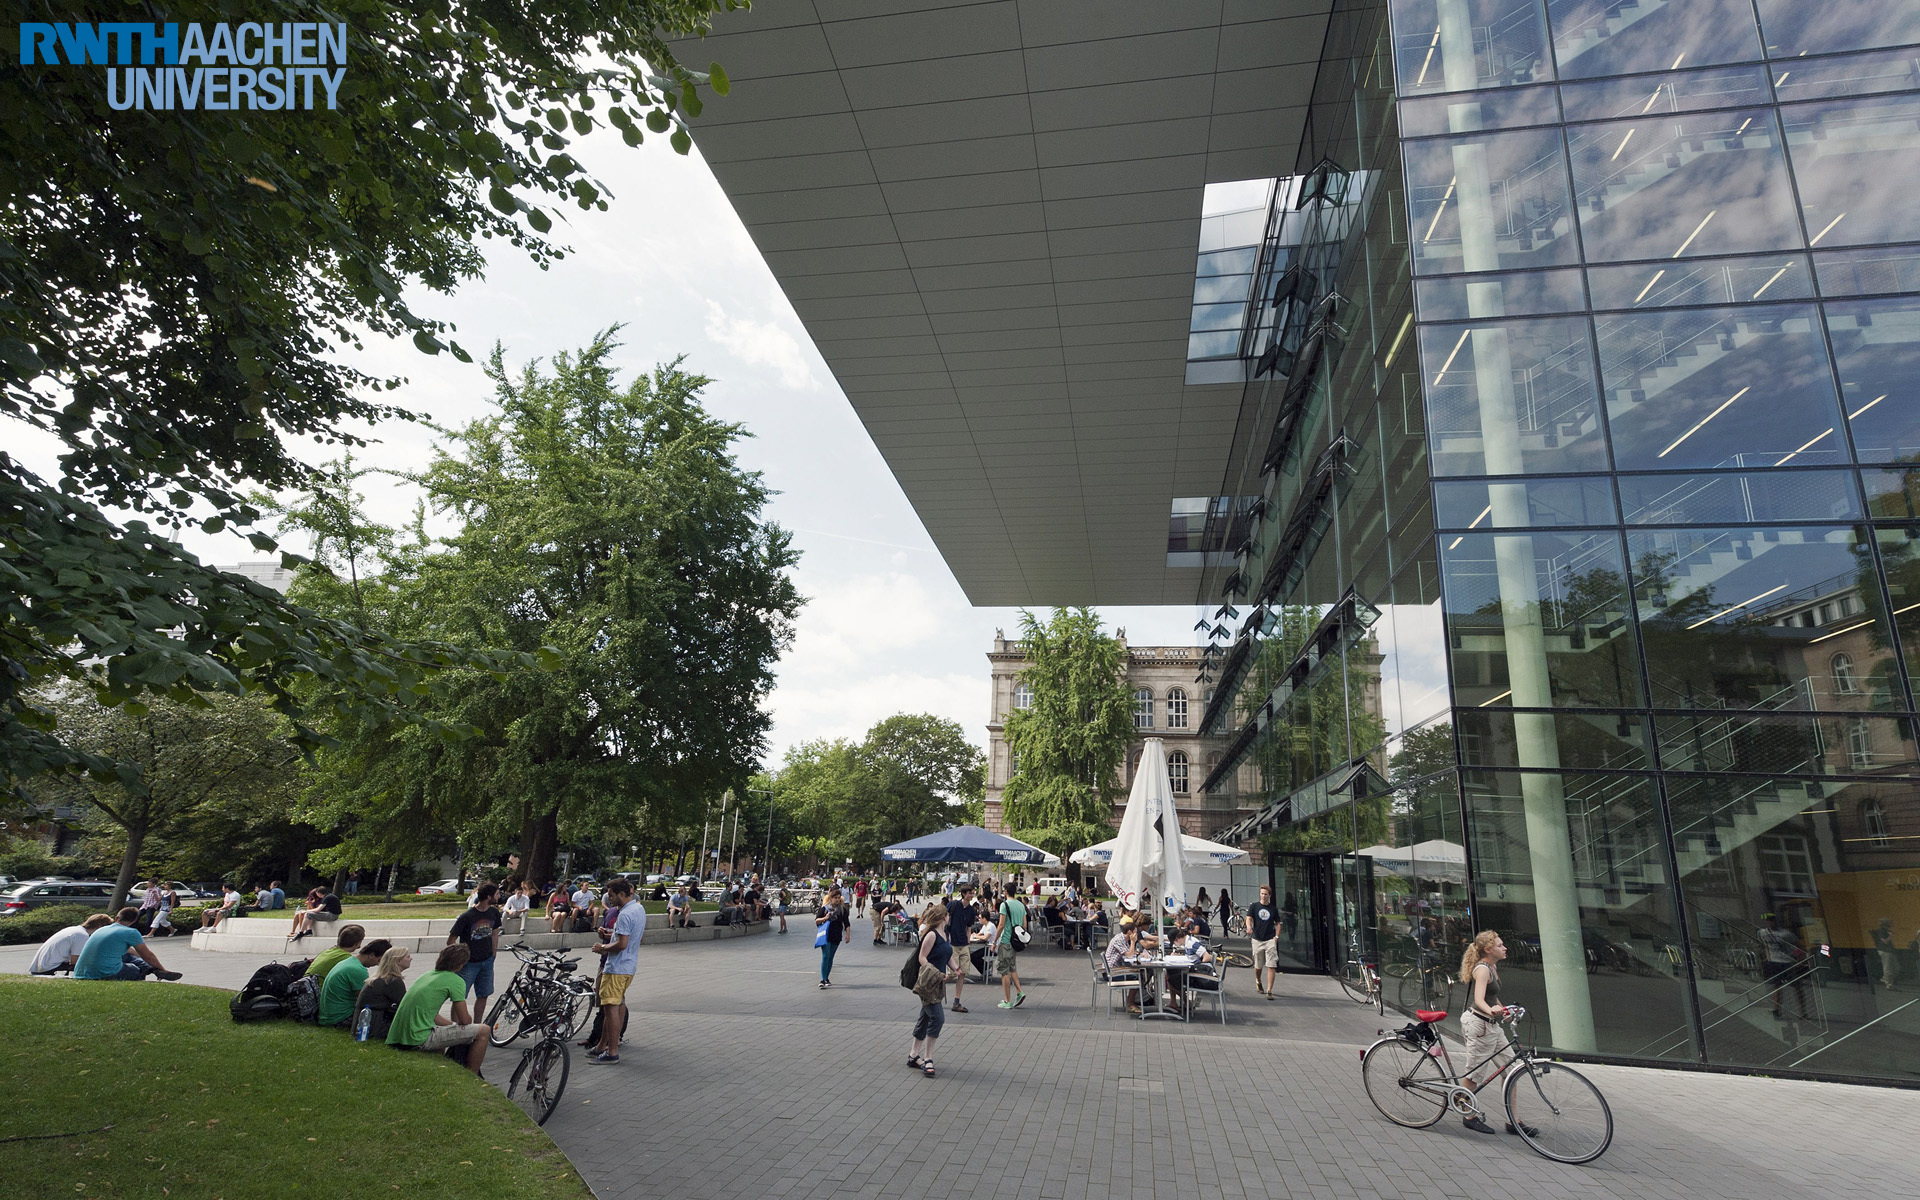
\includegraphics[width = 0.5\textwidth]{Contents/Resources/superc.jpeg}
	\caption[Image (short caption without source)]{Image (detailed caption including source, Source: \cite[1]{Sample.2012})}
	\label{fig:a_image}
\end{figure}

\begin{figure}[htbp]
	\centering
	\begin{subfigure}[t]{0.46\textwidth}
		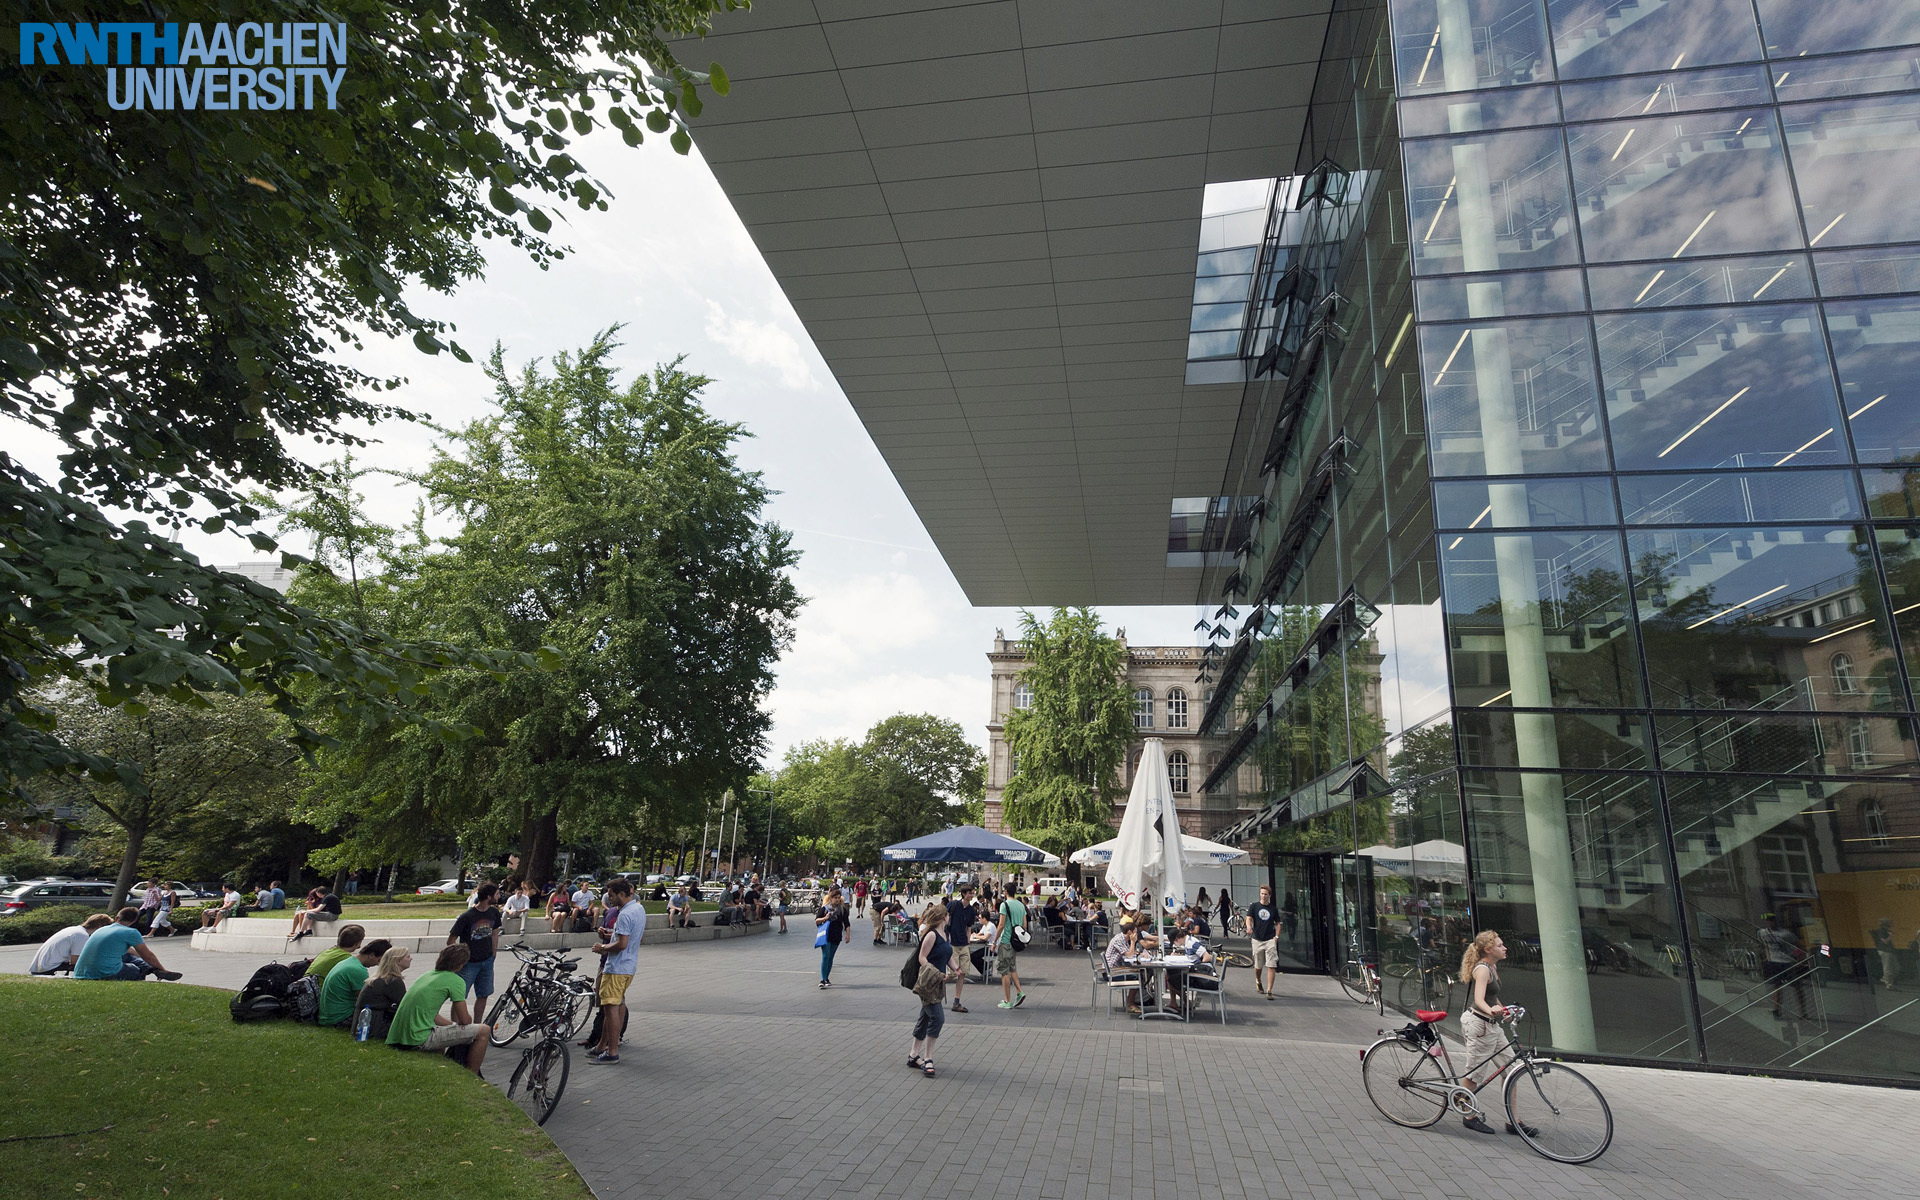
\includegraphics[width = 1\textwidth]{Contents/Resources/superc.jpeg}
		\caption{Image 1}
		\label{fig:image1}
	\end{subfigure}
	\begin{subfigure}[t]{0.46\textwidth}
		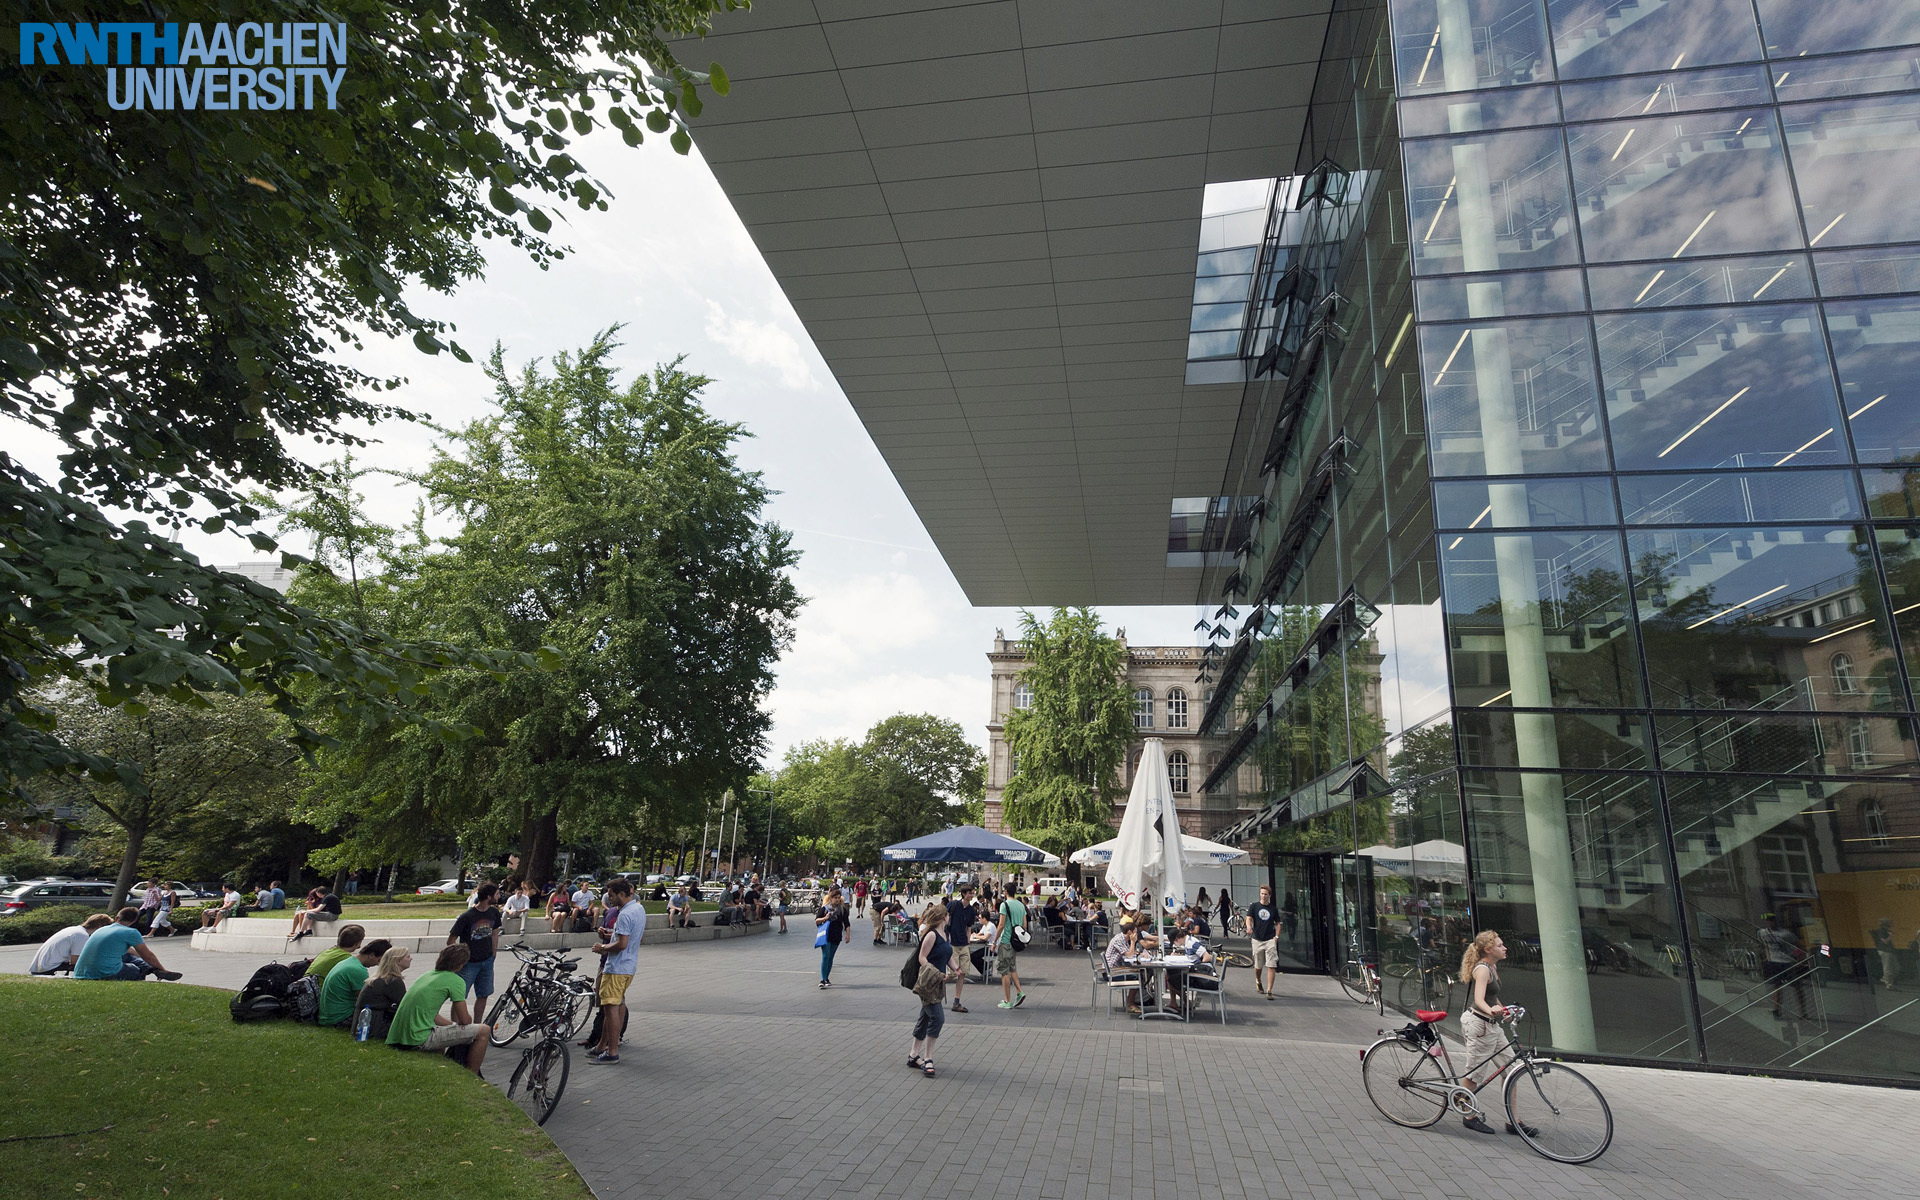
\includegraphics[width = 1\textwidth]{Contents/Resources/superc.jpeg}
		\caption{Image 2}
		\label{fig:image2}
	\end{subfigure}
	\caption[Two images]{Image 1 (a) and Image 2 (b)}
	\label{fig:multiple_images}
\end{figure}

\cleardoublepage
% Section 3 --------------------------------------------------------------
% 		Name of the section
% --------------------------------------------------------------------------
\section{Tables}
\label{sec:tables}

\begin{table}[htbp]
	\centering	
	\caption{Tables with automatic alignment}
		\begin{tabular}{lcr}
	 	\toprule
	 	l & c & r\\
	 	\midrule
		a & b & c\\[0.25em]
		aa & bb & cc\\[0.25em]
		aaa & bbb & ccc\\
		\bottomrule
	\end{tabular}	
	\label{tab:table1}
\end{table}

\begin{table}[htbp]
  \centering
  \caption{Tables aligned to seperators}
    \begin{tabular}{R{4}{3} R{4}{0}}
    \toprule
          \multicolumn{1}{c}{a} & \multicolumn{1}{c}{b}\\
    \midrule
	1,234 & 1234\\
	12,34 & 123\\
	123,4 & 12\\
	1234  & 1\\
    \bottomrule
    \end{tabular}
  \label{tab:table2}
\end{table}

\begin{table}[htbp]
	\centering	
	\caption{Table with multiple cells across various rows and columns}
		\begin{tabular}{lcr}
	 	\toprule
	 	l & c & r\\
	 	\midrule
		\multicolumn{2}{c}{ab} & c\\[0.25em]
		\multirow{2}{*}{aa} & bb & cc\\[0.25em]
		& bbb & ccc\\
		\bottomrule
	\end{tabular}	
	\label{tab:table3}
\end{table}

%\begin{table}[htbp]
%  \centering
%  \caption{multiple sub-tables}
%  \subtable[table 1]{
%    \centering  
%\begin{tabular}{lcr}
%	 	\toprule
%	 	l & c & r\\
%	 	\midrule
%		a & b & c\\[0.25em]
%		aa & bb & cc\\[0.25em]
%		aaa & bbb & ccc\\
%		\bottomrule
%	\end{tabular}	
%  }
%  \subtable[Tabelle 2]{
%    \centering  
%\begin{tabular}{lcr}
%	 	\toprule
%	 	l & c & r\\
%	 	\midrule
%		a & b & c\\[0.25em]
%		aa & bb & cc\\[0.25em]
%		aaa & bbb & ccc\\
%		\bottomrule
%	\end{tabular}	
%  }
%\label{tab:tables}
%\end{table}

\cleardoublepage
% Section 4 --------------------------------------------------------------
% 		Name of the section
% --------------------------------------------------------------------------
\section{Equations}
\label{sec:equations}

\begin{align}
	F = m a 
	\label{eqn:newton_en}
\end{align}


\section{Citation options}

Cite a source: \cite{Sample.2012}\\
Cite a source with a page reference: \cite[12-16]{Sample.2012}\\
Cite multiple Sources: \cites{Samplem.2012}{Samplef.2011}\\
Cite multiple sources with page references: \cites[12-16]{Samplem.2012}[3]{Samplef.2011}\\


% \chapter{Beispielkapitel}
\label{cha:beispielkapitel}
Dieses Beispielkapitel dient der Darstellung häufig verwendeter Elemente in LaTeX wie Aufzählungen, Abbildungen, Tabellen oder Gleichungen. Es hat keinen Anspruch auf Vollständigkeit und kann gerne erweitert werden. Eine ausführliche Beschreibung der LaTeX-Befehle kann der Befehlsübersicht entnommen werden.
Die  Beispiele können kopiert und dann angepasst werden.  
% Abschnitt 1 --------------------------------------------------------------
% 		Name des Abschnittes
% --------------------------------------------------------------------------
\section{Aufzählungen}
\label{sec:aufzaehlungen}

\subsection{Aufzählungen mit Punkten}
\label{aufzaehlung_punkte}

\begin{itemize}
	\item Körper
	\item Bindungselemente
	\item Koppelelemente
\end{itemize}

\subsection{Aufzählungen mit Zahlen}
\label{aufzaehlung_zaheln}

\begin{enumerate}
	\item Körper
	\item Bindungselemente
	\item Koppelelemente
\end{enumerate}

\cleardoublepage
% Abschnitt 2 --------------------------------------------------------------
% 		Name des Abschnittes
% --------------------------------------------------------------------------
\section{Abbildungen}
\label{sec:abbildungen}

\begin{figure}[htbp]
	\centering
		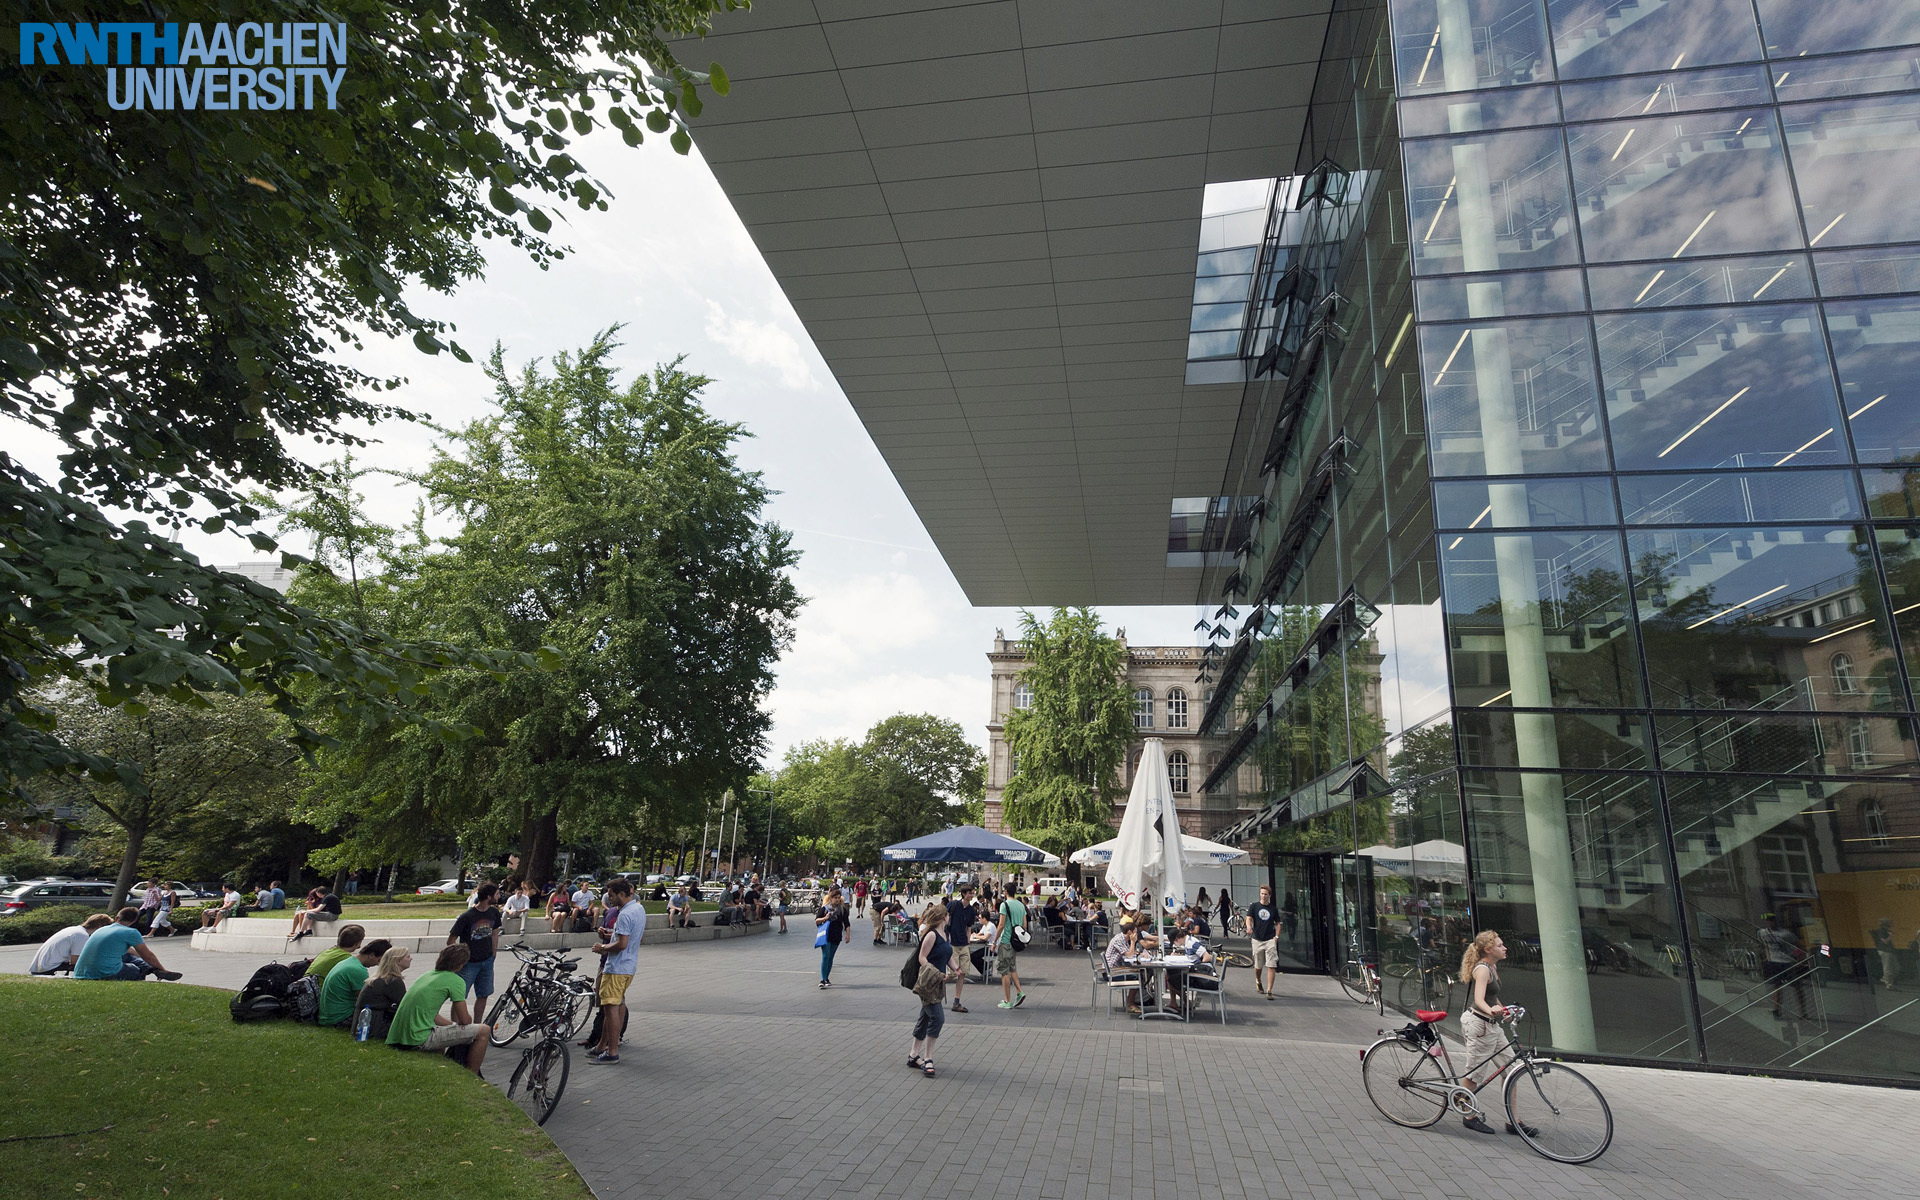
\includegraphics[width = 0.5\textwidth]{Contents/Resources/superc.jpeg}
	\caption[Eine Abbildung (kurze Abbildungsunterschrift ohne Quelle)]{Eine Abbildung (lange Abbildungsunterschrift mit Quelle, Quelle: \cite[1]{Mustermann.2012})}
	\label{fig:eine_abbildung}
\end{figure}

\begin{figure}[htbp]
	\centering
	\begin{subfigure}[t]{0.46\textwidth}
		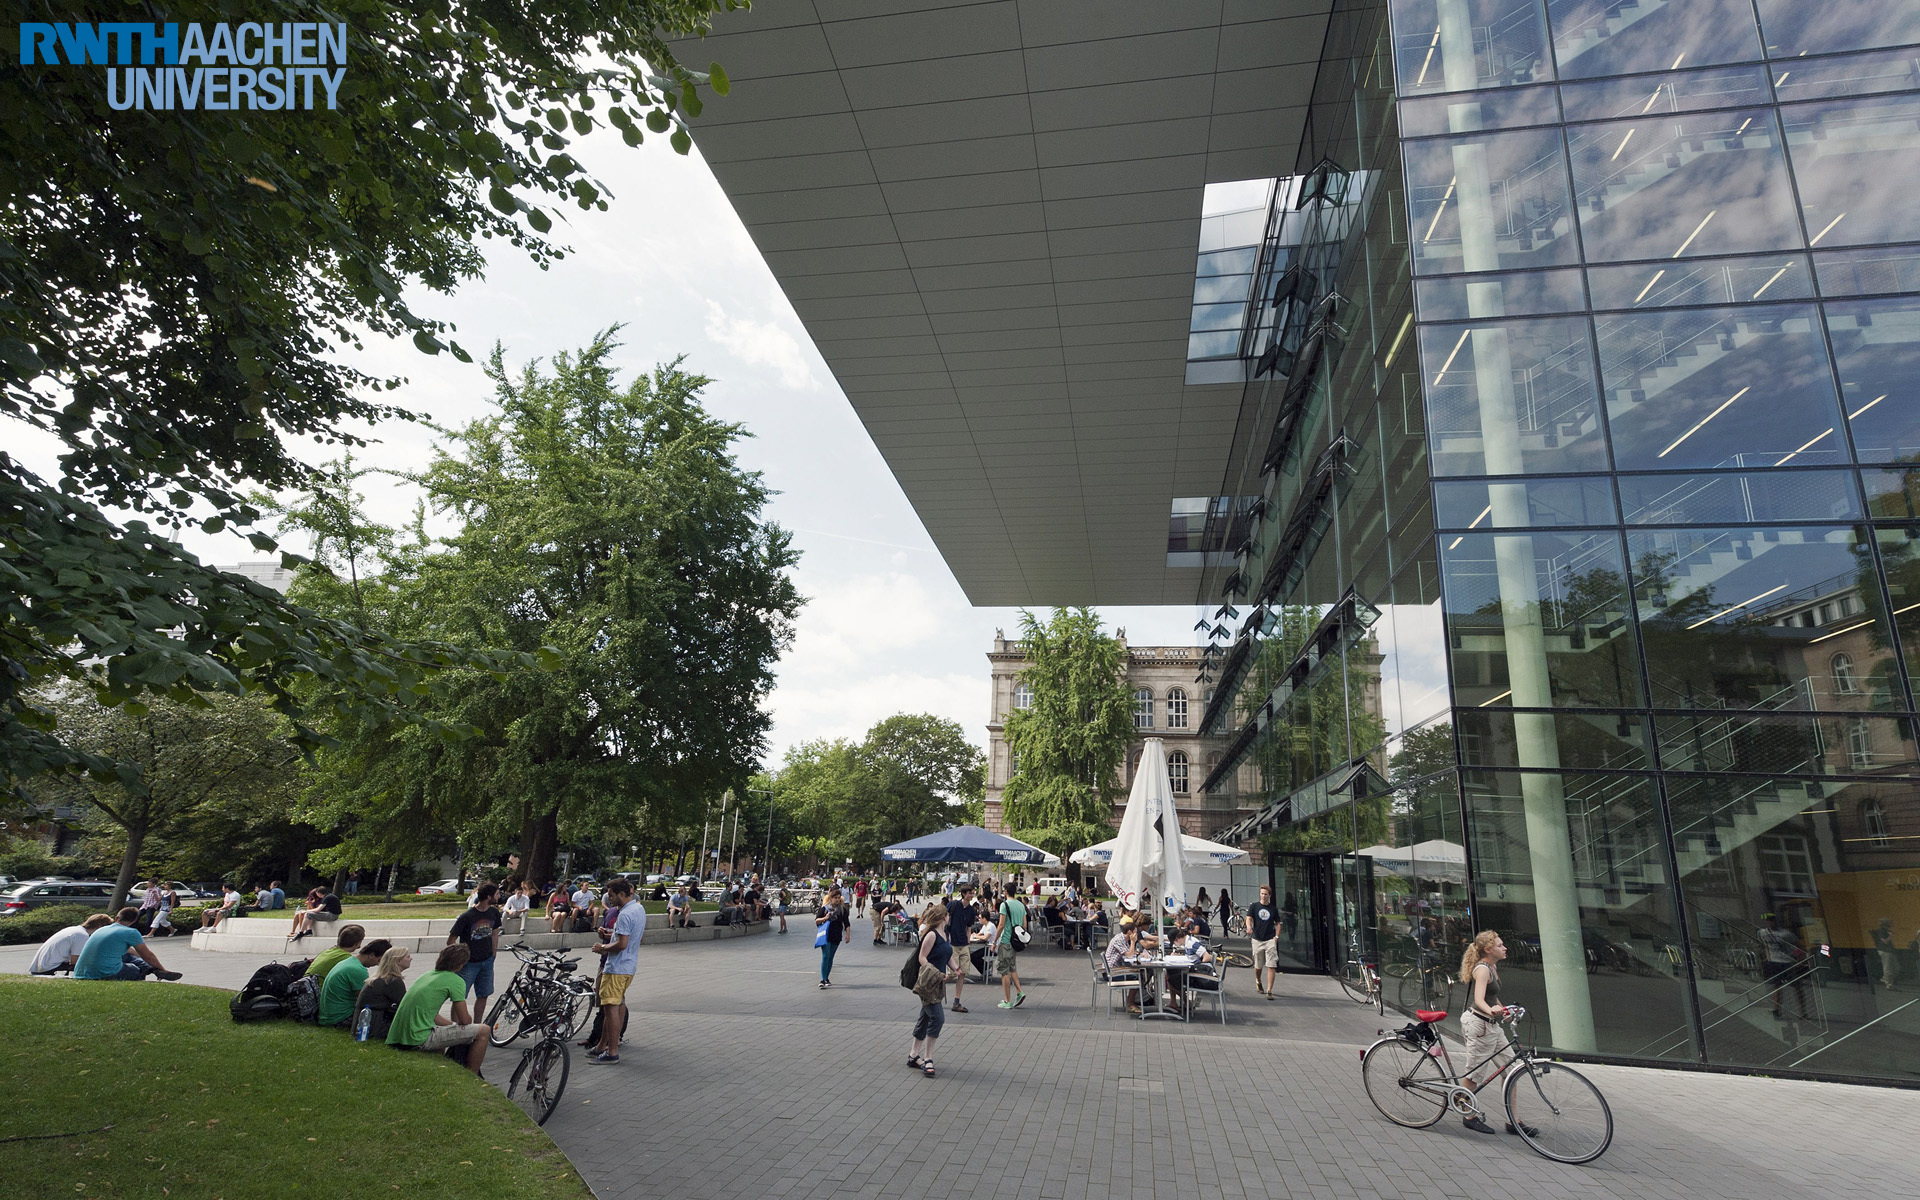
\includegraphics[width = 1\textwidth]{Contents/Resources/superc.jpeg}
		\caption{Bild 1}
		\label{fig:bild1}
	\end{subfigure}
	\begin{subfigure}[t]{0.46\textwidth}
		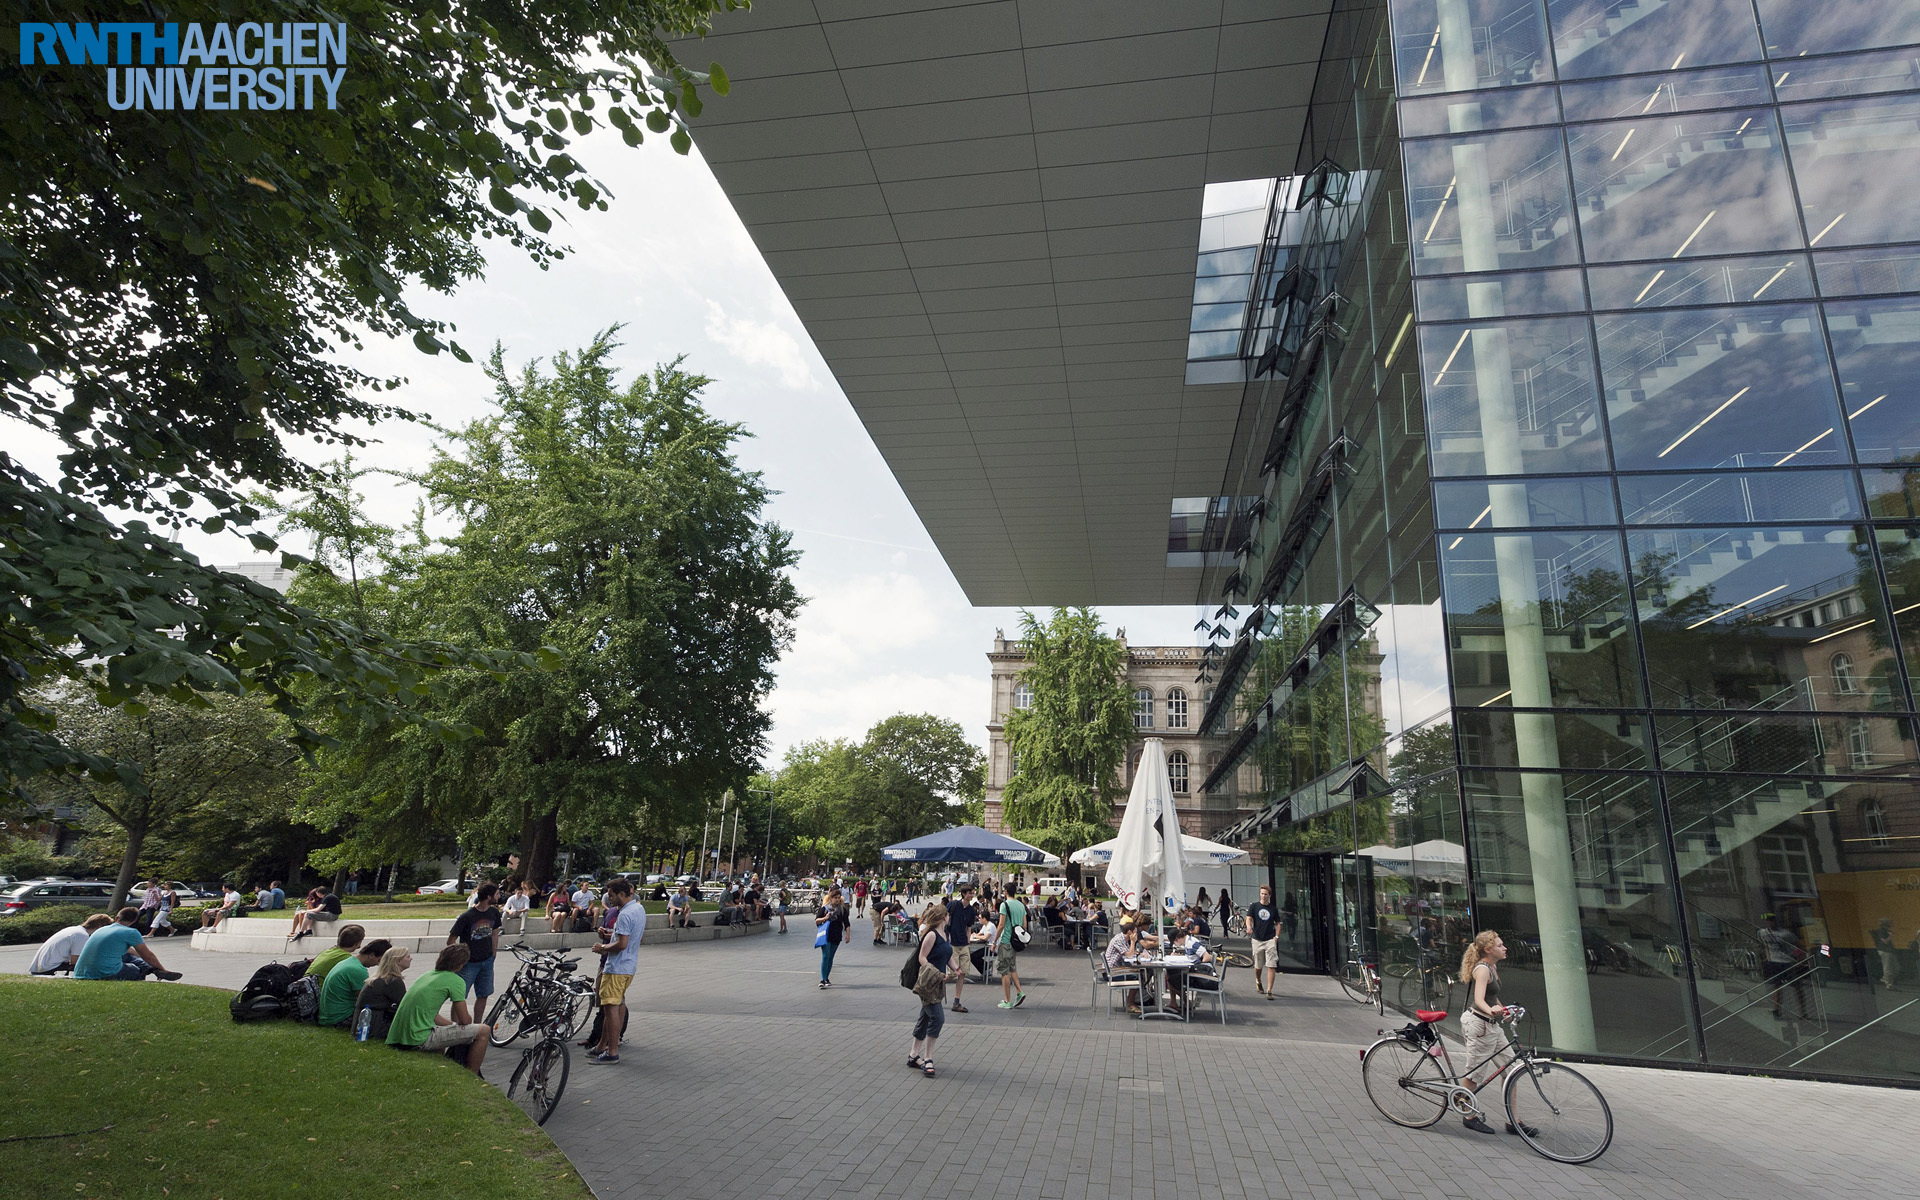
\includegraphics[width = 1\textwidth]{Contents/Resources/superc.jpeg}
		\caption{Bild 2}
		\label{fig:bild2}
	\end{subfigure}
	\caption[Zwei Abbildungen]{Bild 1 (a) und Bild 2 (b)}
	\label{fig:mehrere_abbildungen}
\end{figure}

\cleardoublepage
% Abschnitt 3 --------------------------------------------------------------
% 		Name des Abschnittes
% --------------------------------------------------------------------------
\section{Tabellen}
\label{sec:tabellen}

\begin{table}[htbp]
	\centering	
	\caption{Tabelle mit automatischer Ausrichtung}
		\begin{tabular}{lcr}
	 	\toprule
	 	l & c & r\\
	 	\midrule
		a & b & c\\[0.25em]
		aa & bb & cc\\[0.25em]
		aaa & bbb & ccc\\
		\bottomrule
	\end{tabular}	
	\label{tab:tabelle1}
\end{table}

\begin{table}[htbp]
  \centering
  \caption{Tabelle mit Ausrichtung an Trennungszeichen}
    \begin{tabular}{R{4}{3} R{4}{0}}
    \toprule
          \multicolumn{1}{c}{a} & \multicolumn{1}{c}{b}\\
    \midrule
	1,234 & 1234\\
	12,34 & 123\\
	123,4 & 12\\
	1234  & 1\\
    \bottomrule
    \end{tabular}
  \label{tab:tabelle2}
\end{table}

\begin{table}[htbp]
	\centering	
	\caption{Tabelle mit Zellen über mehrere Zeilen oder Spalten}
		\begin{tabular}{lcr}
	 	\toprule
	 	l & c & r\\
	 	\midrule
		\multicolumn{2}{c}{ab} & c\\[0.25em]
		\multirow{2}{*}{aa} & bb & cc\\[0.25em]
		& bbb & ccc\\
		\bottomrule
	\end{tabular}	
	\label{tab:tabelle3}
\end{table}

%\begin{table}[htbp]
%  \centering
%  \caption{Mehrere Untertabellen}
%  \subtable[Tabelle 1]{
%    \centering  
%\begin{tabular}{lcr}
%	 	\toprule
%	 	l & c & r\\
%	 	\midrule
%		a & b & c\\[0.25em]
%		aa & bb & cc\\[0.25em]
%		aaa & bbb & ccc\\
%		\bottomrule
%	\end{tabular}	
%  }
%  \subtable[Tabelle 2]{
%    \centering  
%\begin{tabular}{lcr}
%	 	\toprule
%	 	l & c & r\\
%	 	\midrule
%		a & b & c\\[0.25em]
%		aa & bb & cc\\[0.25em]
%		aaa & bbb & ccc\\
%		\bottomrule
%	\end{tabular}	
%  }
%\label{tab:tabellen}
%\end{table}

\cleardoublepage
% Abschnitt 4 --------------------------------------------------------------
% 		Name des Abschnittes
% --------------------------------------------------------------------------
\section{Gleichungen}
\label{sec:gleichungen}

\begin{align}
	F = m a 
	\label{eqn:newton}
\end{align}


\section{Anführungszeichen}
\label{sec:anfuehrungszeichen}
Es gibt mehrere Möglichkeiten deutsche Anführungszeichen einzufügen:\\
\glqq test\grqq\\
"`test"'\\

\section{Zitationen}

Zitation einer Quelle: \cite{Mustermann.2012}\\
Zitation einer Quelle mit Seitenangabe: \cite[12-16]{Mustermann.2012}\\
Zitation mehrerer Quellen: \cites{Mustermann.2012}{Musterfrau.2011}\\
Zitation mehrerer Quellen mit Seitenangabe: \cites[12-16]{Mustermann.2012}[3]{Musterfrau.2011}\\



% \chapter{Zusammenfassung}
\label{cha:zusammenfassung}


%
% \chapter{Outlook}\label{cha:outlook}


%       EXTRAS
%		x Title page
%		- Half title??
%		- Issue [last]
%		x Statutory declaration
%		- (Preface)
%		x Table of contents
%		- List of abbreviations
%		- List of symbols

%       MAIN CHAPTERS
%		- Introduction
%		- Chapters
%		- Summary
%		- Outlook

%       EXTRAS
%		- List of literature
%		- List of illustrations
%		- List of tables
%		- Appendix

\chapter{Introduction}\label{cha:introduction}

Motivation for work

\section{Motivation}\label{sec:motivation} 

\chapter{Literature Review}\label{cha:literature}


\section{ROS on Web}\label{sec:ros_on_web}

\section{Web Tools}\label{sec:ros_on_web}

\section{Unreal WASM??}

\chapter{Concept Realization}\label{cha:concept}


\section{Concept}\label{sec:concept}

Ideal scenario: 
- click on a link and run ROS
- connect to a robot via bluetooth
- share simulations and algorithms

\section{Technical Levels}\label{sec:levels}

    \subsection{User Levels of Interaction}\label{sub:user_levels}

    \subsection{Technical Levels of Implementation}\label{sub:tech_levels}

\section{Scope}\label{sec:scope}

    - Middleware replacement (why sockets don't work)

    - JavaScript ``ROS master''


% Too many sections
% Add a note to point or link to issues about the changes
% Thesis will come with a git repo
% Add QR codes to link to specific commit for each step of development
% 1.0 is ready to be published
% Add a note about submitting to ROSCon
% Submit proposal in March

\chapter{Methodology}\label{cha:methodology}

    In the spirit of reproducibility, this chapter describes the tools and procedures used in the development of this project. Starting with the hardware, the requirements for this project were minimal. An Intel\textsuperscript{\textregistered} Core\texttrademark\ i7-1065G7 CPU 1.30 GHz processor with a memory capacity of 16 GiB of RAM was used. The operating system consisted of Ubuntu 22.04. A system with substandard specifications can also be adequate for development.

\section{Development Environment}

    For the sake of simplicity and to isolate the development environment from global dependencies, a \textsf{conda} environment was created. This \textsf{conda} environment was used to build the \ac{ROS} packages required. The essential packages installed in the development environment are shown in Table~\ref{tab:envdeps}. For quick installation, an environment yaml file is provided at TODO

    \begin{table}[htbp]
        \color{textColor}
        \centering	
        \caption{Development environment dependencies}

        \begin{tabular}{lc}
            \toprule
            \textbf{Package} & \textbf{Version} \\
            \midrule
            \textsf{python} & $3.10$ \\

            \textsf{setuptools}\tablefootnote{Version $58.2.0$ of \textsf{setuptools} is the highest version that supports \textsf{setup.py} installs which many of the core ROS packages depend upon.} & $58.2.0$ \\

            \textsf{numpy} & $1.24$ \\ 

            \textsf{lark}\tablefootnote{The \textsf{lark} package is required for \textsf{builtin}\texttt{\_}\textsf{interfaces}} & $1.1$ \\

            \textsf{rosdep} & $0.22$ \\

            \textsf{cmake} & $3.25$ \\

            \textsf{colcon-core} & $0.12$ \\

            \textsf{colcon-ros} & $0.3$ \\

            \textsf{colcon-package-selection} & $0.2$ \\

            \textsf{colcon-devtools} & $0.2$ \\

            \textsf{nodejs} & $18.12$ \\

            \bottomrule
                
        \end{tabular}\label{tab:envdeps}
    \end{table}


\section{Compilation Tools}

    TODO: more details

    Given that the \textsf{colcon} package is already well adapted to build ROS packages, \textsf{colcon} was widely used throughout this project with a few customizations. 


    There are currently four ways to port projects to WebAssembly~\cite{portingwasm}:
    
    \begin{itemize}
        \item Writing WebAssembly directly
        \item Using AssemblyScript
        \item Targeting WebAssembly as output for Rust applications
        \item Using Emscripten for C/C++ applications
    \end{itemize}

    Since most \ac{ROS} 2 packages are written in C/C++, the easiest solution was to use Emscripten. Emscripten is a compiler toolchain which takes C/C++ source code and outputs a wasm module, the JavaScript \textit{glue} code and optionally an \ac{HTML} document, as illustrated in Figure~\ref{fig:emscripten}. In terms of \ac{ROS} packages, for each executable, for example a \textsf{talker.cpp} containing a publisher node, Emscripten will output three files per executable: \textsf{talker.wasm}, \textsf{talker.js} and \textsf{talker.html}.

    \begin{figure}[htbp]
        \centering
        \begin{tikzpicture}
            \node (cpp) [fileBox] {C/C++ \\ source code \\ \footnotesize\textsf{talker.cpp}};
            \node (emsdk) [
                fileBox, 
                right of=cpp, 
                xshift=4cm,
                fill=shade20,
            ] {\textbf{Emscripten}};

            \node (dot) [circle, right of=emsdk, opacity=0, xshift=1.2cm] {\tiny};

            \node (wasm) [fileBox, right of=emsdk, xshift=4cm, yshift=1.2cm] {wasm module \footnotesize\textsf{talker.wasm}};
            
            \node (html) [outerBox, right of=emsdk, xshift=4cm, yshift=-0.2cm, anchor=north] {HTML document \\ \footnotesize\textsf{talker.html}};

            \node (js) [innerBox, below of=html, yshift=0.5cm]{JavaScript \\ ``glue'' code \\ \footnotesize\textsf{talker.js}};

            \draw [arrow] (cpp) -- (emsdk);
            \draw [arrow] (dot.center) |- (wasm);
            \draw [arrow] (dot.center) |- (html);
            \draw [arrow] (dot.center) |- (js);
            \draw [thick] (emsdk.east) -- (dot.center);
            % \draw [decorate, decoration = {brace, amplitude=10pt, aspect=0.6}] (7.7,-3) --  (7.7,2);


        \end{tikzpicture}
        \caption{Transformation of C/C++ code to WebAssembly through Emscripten~\cite{portingwasm}.}
        \label{fig:emscripten}
    \end{figure}

    In order to cross-compile the packages to WebAssembly, the \ac{emsdk} version $3.1$ was installed. The Emscripten toolchain was then provided to \textsf{colcon} as a \textsf{cmake} argument (See Appendix~\ref{sec:apxblasm} Line $109$).


\section{Package Building Process}

    Before any packages could be built, all of the ROS 2 core packages were cloned in a local workspace. To prevent compilation issues, packages related to the default middleware implementations were excluded by adding a \textsf{COLCON}\texttt{\_}\textsf{IGNORE} file in their respective root directories; these include \textsf{iceoryx}, \textsf{cyclonedds}, \textsf{fastrtps}, and \textsf{connextdds}. A secondary purpose for excluding these packages is to ensure that the custom middleware implementation is the only implementation available at runtime. This custom middleware implementation must also be included in the current workspace before proceeding. 

    Additionally, a ``blasm'' script was created to aid in the building of packages given that the number of arguments quickly became exceedingly lengthy for manual input. The entire script is included in Appendix~\ref{sec:apxblasm} for reference. With this script, it is possible to build any package and its dependencies, or to build a package individually. Care must be taken to ensure that the environment variables for the tools such as \textsf{EMSDK}\texttt{\_}\textsf{DIR} are set accordingly. The list of options for this script are shown in Figure~\ref{fig:blasm}.

    \begin{figure}[htbp]
        \centering
        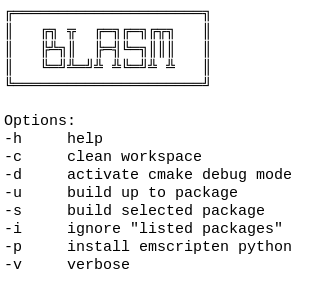
\includegraphics[width=0.4\textwidth]{04_blasm.png}
        \caption{Blasm script options.}
        \label{fig:blasm}
    \end{figure}


    If the package compiles without errors, any executables in the package will be converted to \textit{.wasm} and \textit{.js} files to be run on the browser.


\section{Debugging Tools}

    When working with new ROS packages, there are two main sources of errors: errors during compilation and errors at runtime. To tackle compilation errors, the first step is to obtain a full description of the error. The ``blasm'' script has the option to dynamically activate verbose (\textsf{-v}) mode as needed.

    Secondly, for debugging errors at runtime, one of the most effective tools is the use of logs. Core \ac{ROS} packages such as \textsf{rcutils} and \textsf{rcpputils} already include logging functionalities. Adapting these \ac{ROS} logs into any newly created packages allows for efficient and quick debugging. Alternatively, customized logging functions could be implemented for an in-depth analysis at the expense of increasing the complexity of the package in question.

\section{Post Processing}

    Once the executables have been successfully compiled, the generated JavaScript files are augmented with additional functions to enable communication between the main thread and the ROS packages. The added functions are described in Appendix~\ref{sec:apxmodule}. (TODO: OR provide link to file on GitHub)

\section{Testing Environment}

    Lastly, there are two phases of testing. The first phase consists of testing the packages directly from the terminal. For the early stages such as during the replacement of the middleware implementation, cross-compilation is not yet required; thus, it is possible to locally test the middleware packages by comparing their behavior with the default middleware implementations. This can be achieved in a separate \textsf{conda} environment with \ac{ROS} 2 packages preinstalled by creating and installing an overlay which only includes the customized middleware implementation.

    And the second phase involves testing the packages on a web browser. For this project, only Firefox and Chrome were subject to testing due to their popularity. The tools developed in this project may be suitable for other browsers, however, their full functionality is not guaranteed.


\subsection{Package Management and Distribution}

    TODO:
    - Automating package building
    - Pipelines
    - robostack?

\chapter{Middleware}

    A significant change from \ac{ROS} 1 to \ac{ROS} 2 is the shift from a custom transport layer consisting of \ac{TCPROS} to \ac{DDS}. \ac{DDS} is a publish-subscribe communication standard defined by \ac{OMG}. \ac{DDS} uses \ac{IDL} for defining and serializing messages~\cite{rosondds}. In contrast to \ac{ROS} 1, which requires a \ac{ROS} master in order for nodes to discover and communicate with each other, \ac{ROS} 2 discovery system is handled by \ac{DDS} and each of the \ac{DDS} vendors provides different options for customizing the communication layer.

    One notable advantage of moving away from a custom transport protocol is that the \ac{ROS} client libraries are now agnostic to the middleware interface; this means that the complexities of the \ac{DDS} implementation are not exposed to the end user~\cite{ros2middle}. As a consequence, multiple middleware interfaces can be implemented as long as they fulfill the following requirements: 
    \begin{itemize}
        \item publishing and subscribing
        \item message serialization
        \item discovery
    \end{itemize}\label{ite:rmwreqs}
    
    The interaction between the \ac{ROS} user, the \ac{ROS} client libraries, and the middleware layers is shown in Figure~\ref{fig:middleware}.

    \begin{figure}[htbp]
        \centering
        \vspace{1em}
        \begin{tikzpicture}
            \node (user) [packBox] {ROS User};

            \node (rcl) [packBox, yshift=-2cm] {ROS Client Libraries \\ \small\textsf{rclcpp | rclpy}};

            \node (interface) [packBox, yshift=-4cm] {Middleware Interface \\ \small\textsf{rmw}};

            \node (implementation) [packBox, yshift=-6cm] {\textbf{Middleware Implementation} \\ \small\textsf{fastrtps | cyclonedds | connextdds | gurumdds | custom}};

            \begin{scope}[transform canvas={xshift=-0.5cm}]
                \draw [-to] (user) -- (rcl);
                \draw [-to] (rcl) -- (interface);
                \draw [-to] (interface) -- (implementation);
            \end{scope}

            \begin{scope}[transform canvas={xshift=0.5cm}]
                \draw [to-] (user) -- (rcl);
                \draw [to-] (rcl) -- (interface);
                \draw [to-] (interface) -- (implementation);
            \end{scope}

        \end{tikzpicture}
        \vspace{1em}
        \caption{Relations between the user, the \ac{ROS} client libraries and the middleware packages~\cite{ros2middle}.}
        \label{fig:middleware}
    \end{figure}


\section{Supported Implementations}

    Currently, \ac{ROS} 2 releases provide full support for three middleware implementations: eProsima Fast \ac{DDS}, Eclipse Cyclone \ac{DDS}, and \ac{RTI} Connext \ac{DDS}. The binaries also support Gurum \ac{DDS}, but the implementation requires a separate installation~\cite{docsdds}. 

    \subsection{eProsima Fast DDS}

    eProsima Fast \ac{DDS}, also known as Fast \ac{RTPS}, is the default middleware implementation for \ac{ROS} 2 packages. Some of the main advantages of Fast \ac{DDS} is that it is free, open source, and it is developed for most platforms including Linux, Windows, Mac OS, and QNX. A rich set of \ac{QoS} parameters is also available for tuning the communication protocols to any particular system. Fast \ac{DDS} follows a \ac{DCPS} model, which consists four elements: publishers, subscribers, topics, and domains~\cite{dcps}. This model introduces the concept of \textsf{Data Writers} and \textsf{Data Readers} which, as the names imply, have read and write permissions to the ``Global Data Space'' as specified by the \ac{DDS} standard~\cite{introdds}. Figure~\ref{fig:ddsdomain} displays an example of the Fast \ac{DDS} architecture and demonstrates how the different elements interact with each other.

    \begin{figure}[htbp]
        \centering
        \vspace{1em}
        \begin{tikzpicture}
            \node (domain) [
                box, 
                minimum width=14cm,
                text depth=6cm,
                fill=igmrLightBlue!10!bgColor,
            ] {DDS Domain};
            
            \node (p1) [
                box,
                xshift=-4cm,
                minimum width = 4cm,
                text depth=4.5cm,
                fill=igmrLightBlue!40!bgColor,
            ] {Domain Participant};

            \node (pub1) [
                box,
                xshift=-4cm,
                yshift=0.5cm,
                minimum width=3.5cm,
                text depth=1cm
            ] {Publisher};

            \node (dw1) [
                box,
                xshift=-4cm,
                yshift=0.2cm,
                minimum width=3cm,
                fill=bgColor,
            ] {Data Writer};

            \node (sub1) [
                box,
                xshift=-4cm,
                yshift=-1.5cm,
                minimum width=3.5cm,
                text depth=1cm
            ] {Subscriber};

            \node (dr1) [
                box,
                xshift=-4cm,
                yshift=-1.8cm,
                minimum width=3cm,
                fill=bgColor,
            ] {Data Reader};

            \node (p2) [
                box,
                xshift=4cm,
                minimum width=4cm,
                text depth=4.5cm,
                fill=igmrLightBlue!40!bgColor,
            ] {Domain Participant};

            \node (sub2) [
                box,
                xshift=4cm,
                yshift=0.5cm,
                minimum width=3.5cm,
                text depth=1cm
            ] {Subscriber};

            \node (dr2) [
                box,
                xshift=4cm,
                yshift=0.2cm,
                minimum width=3cm,
                fill=bgColor,
            ] {Data Reader};

            \node (t1) [
                box,
                minimum width=2cm,
                minimum height=1cm,
                fill=igmrLightBlue!40!bgColor,
            ] {Topic};

            \node (dot1) [
                rectangle,
                xshift=-1.5cm,
            ] {};

            \draw [thick] (t1) -- (dot1.center);
            \draw [arrow] (dw1.east) -- (dw1.east-|t1.west);
            \draw [arrow] (dot1.center) |- (dr1);
            \draw [arrow] (t1.east|-dr2.west) -- (dr2.west);

        \end{tikzpicture}
        \vspace{1em}
        \caption{Instance of a typical Fast \ac{DDS} domain model.}
        \label{fig:ddsdomain}
    \end{figure}

    \subsection{Eclipse Cyclone DDS}

        Similar to Fast \ac{DDS}, Cyclone \ac{DDS} is free and open source and supports the three major platforms, Linux, Windows, and Mac OS. Cyclone \ac{DDS} offers a ``data-centric'' architecture with space- and time-decoupling with a zero configuration discovery system~\cite{eclipse}. Additionally, this implementation includes Python bindings to simplify the definition of data types. 

    \subsection{RTI Connext DDS}

        Unlike the previously mentioned \ac{DDS} implementations, \ac{RTI} Connext DDS requires a separate installation plus the purchase of a license, however, free licenses are available for researchers and academics~\cite{connextuni}. \ac{RTI} also offers a variety of tools to \ac{ROS} users including admin consoles, system monitors, and recording and routing services~\cite{rtiblog}.

    \subsection{Gurum Networks Gurum DDS}

        The last implementation which is supported by the \ac{ROS} 2 binaries is GurumDDS. And as in the case of Connext DDS, GurumDDS also requires its own installation after the purchase of a license, although, free trials are available~\cite{gurum}. 


\section{Custom Middleware}

    Out of the aforementioned middleware implementations, none of them have targeted the web browser as the basis for the \ac{DDS} Global Data Space. There exists a \ac{WebDDS} standard, also specified by \ac{OMG}, which dictates how a \ac{DDS} system can be exposed to web clients via a \ac{WebDDS} service~\cite{webdds}. However, this setup would still require a native \ac{DDS} system. As an alternative to \ac{DDS}, custom middleware packages can be implemented as long as they meet the basic requirements listed in Section~\ref{ite:rmwreqs}.

    \subsection{Email}

        An excellent example of a middleware implementation which is not based on the \ac{DDS} standard is \textsf{rmw\_email}. With this implementation, all of the \ac{ROS} 2 communications for publishing and subscribing to topics and to call and respond to services are handled by sending emails. 

        \begin{figure}[htbp]
            \centering
            \begin{subfigure}[t]{0.49\textwidth}
                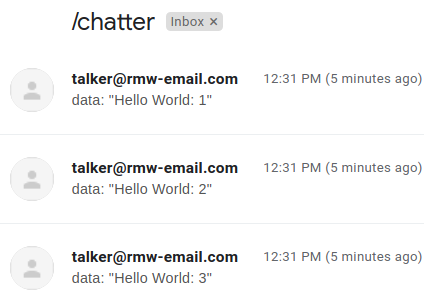
\includegraphics[height=0.68\textwidth]{05_email_pub.png}
                \caption{Email publisher}
            \end{subfigure}
            \begin{subfigure}[t]{0.49\textwidth}
                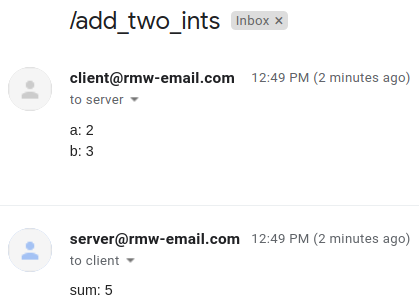
\includegraphics[height=0.68\textwidth]{05_email_srv.png}
                \caption{Email service client and server}
            \end{subfigure}
            \vspace{1em}
            \caption{Email \ac{RMW} implementation.}
            \label{fig:email}
        \end{figure}

        The implementation consists of two parts: \textsf{email} for handling the communications and \textsf{rmw\_email} which acts as an adapter to interface with \textsf{rmw}~\cite{emailblog}. Figure~\ref{fig:email} shows a \ac{ROS} publisher, a service client, and a service server using this \textsf{email} middleware. Although \textsf{rmw\_email} does not reach the level of performance of the standard \ac{DDS} implementations, it showcases the flexibility of the additional abstraction layer integrated in \ac{ROS} 2 to support various middleware designs.


    \subsection{Zenoh}

        Continuing the trend of non-\ac{DDS} middleware implementations, another approach involves the use of Eclipse Zenoh. Zenoh is a publication, subscription and query protocol to unify data which can be used in embedded micro-controllers or even data centers~\cite{zenoh}. Open Robotics has tested the potential of using Zenoh as a middleware for ROS 2 applications and concluded that it could alleviate some of the common problems encountered with the default \ac{DDS} implementations by providing the users with hassle-free experience which does not require configuration and tuning unlike its \ac{DDS} counterparts~\cite{ros2zenoh}.

        Similar to \textsf{rmw\_email}, the interface between Zenoh and \ac{ROS} 2 is handled by \textsf{rmw\_zenoh}. As of 2023, \textsf{rmw\_zenoh} still remains in the experimental phase. One notable aspect of this implementation, is the adaptation of Fast CDR to provide type support for Zenoh.

    \subsection{Minimal Middleware Implementation}

        The development of a custom middleware implementations consist of two major parts: the creation of a middleware ``adapter'' to communicate with the \ac{ROS} 2 middleware interface, and the formation of the middleware implementation itself. An overview of a custom middleware architecture is demonstrated in Figure~\ref{fig:rmwarch}. 

        \begin{figure}[htbp]
            \centering
            \vspace{1em}
            \begin{tikzpicture}
                \node (rmw) [packBox] {ROS 2 Middleware Abstraction Interface \\ \small\textsf{rmw}};

                \node (custom) [
                    rectangle,
                    rounded corners,
                    yshift=-3.5cm,
                    minimum width=12cm,
                    text width=11.5cm,
                    text height=4.5cm,
                    draw=textColor,
                    align=justify,
                    fill=igmrLightBlue!10!bgColor,
                ] {Custom Middleware};

                \node (rmwwasm) [
                    packBox, 
                    yshift=-2.3cm,
                    fill=igmrLightBlue!40!bgColor,
                ] {Middleware Adapter \\ \small\textsf{rmw\_email | rmw\_zenoh | rms\_wasm}};

                \node (interface) [
                    packBox, 
                    yshift=-4.3cm,
                    fill=igmrLightBlue!40!bgColor,
                ] {Middleware Implementation \\ \small\textsf{Email | Zenoh | Web Browser}};

                \begin{scope}[transform canvas={xshift=-0.5cm}]
                    \draw [arrow] (rmw) -- (rmwwasm);
                    \draw [arrow] (rmwwasm) -- (interface);
                \end{scope}

                \begin{scope}[transform canvas={xshift=0.5cm}]
                    \draw [arrow] (rmwwasm) -- (rmw);
                    \draw [arrow] (interface) -- (rmwwasm);
                \end{scope}

            \end{tikzpicture}
            \vspace{1em}
            \caption{Architecture overview of a \ac{ROS} 2 custom middleware implementation.}
            \label{fig:rmwarch}
        \end{figure}

        There are no standardized guidelines for how the middleware implementation should be formatted or what platforms it should support. The design of the implementation is highly dependent on the use case of the \ac{ROS} application. The only design requirements are that the implementation should have the means to publish and subscribe data, perform message serialization from and to \ac{ROS} message types, and have a discovery system to detect other participants in the specified domain. For this project, all of the communications are handled by the web browser and thus, the middleware is implemented in JavaScript.

        For the creation of a middleware ``adapter,'' \textsf{rmw} provides a set of primitives which are needed for higher level \ac{ROS} \ac{API}s. Generating the adapter requires implementing all of the relevant interface functions defined by \textsf{rmw}. Figures~\ref{fig:funinit} through~\ref{fig:funclient} highlight a few of the necessary interface functions. 

        \lstset{
            columns=fullflexible,
            numbers=none,
            backgroundcolor=\color{lightgray!15!bgColor},
            xleftmargin=10pt,
            xrightmargin=10pt,
            frame=lrtb,
            framesep=10pt,
            framerule=0pt,
            % emph={int,char,double,float,unsigned,void,bool,const,uint,string},
            % emphstyle=\color{blue},
            emph={
                rmw_context_t, 
                rmw_ret_t, 
                rmw_init_options_t,
                rmw_node_t,
                rmw_guard_condition_t,
                size_t,
                rmw_publisher_t,
                rmw_publisher_allocation_t,
                rmw_publisher_options_t,
                rmw_qos_profile_t,
                rosidl_message_type_support_t,
                rmw_subscription_t,
                rmw_subscription_allocation_t,
                rmw_subscription_options_t,
                },
            emphstyle=\color{gray!60!black},
        }


        \begin{figure}[htbp]
            \begin{lstlisting}[language=C++]
// Return a zero initialized context structure
rmw_context_t 	rmw_get_zero_initialized_context (void) {...}

// Initialize the middleware with the given options and yield a context
rmw_ret_t 	rmw_init (
    const rmw_init_options_t *options, 
    rmw_context_t *context) {...}
    
// Shutdown the middleware for a given context
rmw_ret_t 	rmw_shutdown (rmw_context_t *context) {...}

// Finalize a context
rmw_ret_t 	rmw_context_fini (rmw_context_t *context) {...}

// Return a zero initialized init options structure
rmw_init_options_t 	rmw_get_zero_initialized_init_options (void) {...}

// Initialize given init_options with the default values and implementation specific values
rmw_ret_t 	rmw_init_options_init (
    rmw_init_options_t *init_options, 
    rcutils_allocator_t allocator) {...}

// Copy the given source init options to the destination init options
rmw_ret_t 	rmw_init_options_copy (
    const rmw_init_options_t *src, 
    rmw_init_options_t *dst) {...}

// Finalize the given init_options
rmw_ret_t 	rmw_init_options_fini (rmw_init_options_t *init_options) {...}\end{lstlisting}
            \caption{Functions for initialization and shutdown.}
            \label{fig:funinit}
        \end{figure}


        \begin{figure}[htbp]
            \begin{lstlisting}[language=C++]
// Create a node and return a handle to that node
rmw_node_t * 	rmw_create_node (
    rmw_context_t *context, 
    const char *name, 
    const char *namespace_, 
    size_t domain_id, 
    bool localhost_only) {...}

// Finalize a given node handle, reclaim the resources, and deallocate the node handle
rmw_ret_t 	rmw_destroy_node (rmw_node_t *node) {...}

// Return a guard condition which is triggered when the ROS graph changes
const rmw_guard_condition_t * 	rmw_node_get_graph_guard_condition (
    const rmw_node_t *node) {...}
\end{lstlisting}
            \label{fig:funnode}
            \caption{Node functions.}
        \end{figure}


        \begin{figure}[htbp]
            \begin{lstlisting}[language=C++]
// Create and return an rmw publisher
rmw_publisher_t * 	rmw_create_publisher (
    const rmw_node_t *node, 
    const rosidl_message_type_support_t *type_support, 
    const char *topic_name, 
    const rmw_qos_profile_t *qos_policies, 
    const rmw_publisher_options_t *publisher_options) {...}

// Destroy publisher
rmw_ret_t 	rmw_destroy_publisher (
    rmw_node_t *node, 
    rmw_publisher_t *publisher) {...}

// Initialize a publisher allocation to be used with later publications
rmw_ret_t 	rmw_init_publisher_allocation (
    const rosidl_message_type_support_t *type_support, 
    const rosidl_runtime_c__Sequence__bound *message_bounds, rmw_publisher_allocation_t *allocation) {...}

// Destroy a publisher allocation object
rmw_ret_t 	rmw_fini_publisher_allocation (
    rmw_publisher_allocation_t *allocation) {...}

// Return a rmw_publisher_options_t initialized with default values
rmw_publisher_options_t 	rmw_get_default_publisher_options (void) {...}

// 	Publish a given ros_message
rmw_ret_t 	rmw_publish (
    const rmw_publisher_t *publisher, 
    const void *ros_message, 
    rmw_publisher_allocation_t *allocation) {...}
\end{lstlisting}
            \caption{Publisher functions.}
            \label{fig:funpub}
        \end{figure}


        \begin{figure}[htbp]
            \begin{lstlisting}[language=C++]
// Create and return an rmw subscription
rmw_subscription_t * 	rmw_create_subscription (
    const rmw_node_t *node, 
    const rosidl_message_type_support_t *type_support, 
    const char *topic_name, 
    const rmw_qos_profile_t *qos_policies, 
    const rmw_subscription_options_t *subscription_options) {...}

// Destroy subscription
rmw_ret_t 	rmw_destroy_subscription (
    rmw_node_t *node, 
    rmw_subscription_t *subscription) {...}

// Retrieve the number of matched publishers to a subscription
rmw_ret_t 	rmw_subscription_count_matched_publishers (
    const rmw_subscription_t *subscription, 
    size_t *publisher_count) {...}

// Retrieve the actual qos settings of the subscription
rmw_ret_t 	rmw_subscription_get_actual_qos (
    const rmw_subscription_t *subscription, 
    rmw_qos_profile_t *qos) {...}

// Take an incoming message from a subscription
rmw_ret_t 	rmw_take (
    const rmw_subscription_t *subscription, 
    void *ros_message, 
    bool *taken, 
    rmw_subscription_allocation_t *allocation) {...}
\end{lstlisting}
            \caption{Subscriber functions.}
            \label{fig:funsub}
        \end{figure}

        \begin{figure}[htbp]
            \begin{lstlisting}[language=C++]
// Create an rmw service server that responds to requests
rmw_service_t * 	rmw_create_service (
    const rmw_node_t *node, 
    const rosidl_service_type_support_t *type_support, 
    const char *service_name, 
    const rmw_qos_profile_t *qos_policies) {...}

// 	Destroy and unregister the service from this node
rmw_ret_t 	rmw_destroy_service (
    rmw_node_t *node, 
    rmw_service_t *service) {...}

// Attempt to take a request from this service's request buffer
rmw_ret_t 	rmw_take_request (
    const rmw_service_t *service, 
    rmw_service_info_t *request_header, 
    void *ros_request, 
    bool *taken) {...}

// 	Send response to a client's request
rmw_ret_t 	rmw_send_response (
    const rmw_service_t *service, 
    rmw_request_id_t *request_header, 
    void *ros_response) {...}
\end{lstlisting}
            \caption{Service server functions.}
            \label{fig:funsrv}
        \end{figure}


        \begin{figure}[htbp]
            \begin{lstlisting}[language=C++]
// Create an rmw client to communicate with the specified service
rmw_client_t * 	rmw_create_client (
    const rmw_node_t *node, 
    const rosidl_service_type_support_t *type_support, 
    const char *service_name, 
    const rmw_qos_profile_t *qos_policies) {...}

// Destroy and unregister a service client
rmw_ret_t 	rmw_destroy_client (
    rmw_node_t *node, 
    rmw_client_t *client) {...}

// Send a service request to the rmw server
rmw_ret_t 	rmw_send_request (
    const rmw_client_t *client, 
    const void *ros_request, 
    int64_t *sequence_id) {...}

// Attempt to get the response from a service request
rmw_ret_t 	rmw_take_response (
    const rmw_client_t *client, 
    rmw_service_info_t *request_header, 
    void *ros_response, 
    bool *taken) {...}

// Check if a service server is available for the given service client
rmw_ret_t 	rmw_service_server_is_available (
    const rmw_node_t *node, 
    const rmw_client_t *client, 
    bool *is_available) {...}
\end{lstlisting}
            \caption{Service client functions.}
            \label{fig:funclient}
        \end{figure}


    \pagebreak
    Besides the essential functions for creating and destroying nodes, publishers, subscribers, and services, there exists additional functions to handle events, wait sets, guard conditions, \ac{QoS} policies, and allocators. Additionally, there are utility functions and macros for handling errors, customizing log outputs and name validation. A full list of functions can be found in the \textsf{rmw} \ac{API} documentation~\cite{rmwapi} TODO: or appendix??.

\pagebreak
\section{Substituting ROS 2 Middleware}

    There are two methods of using a particular middleware implementations when launching \ac{ROS} applications other than the default implementation. The first method requires setting the environment variable \small\textsf{RMW\_IMPLEMENTATION} to the implementation identifier of choice. An example of how to launch a publisher node with this method is shown in Figure~\ref{fig:envrmw}.

    \begin{figure}[thbp]
        \centering
            \begin{lstlisting}[
                language=bash,
                frame=lrtb,
                framesep=10pt,
                framerule=0pt,
                emph={RMW_IMPLEMENTATION},
                emphstyle=\color{blue},
            ]
RMW_IMPLEMENTATION=rmw_connextdds ros2 run demo_nodes_cpp talker
\end{lstlisting}
        \caption{Launching a node with Connext \ac{DDS}.}
        \label{fig:envrmw}
    \end{figure}

    Nonetheless, the caveat of this first method is that the \ac{ROS} 2 binaries installed must have support for the specified implementation~\cite{subrmw}. Alternatively, the second method involves rebuilding all of the desired \ac{ROS} 2 packages from source and specify the \small\textsf{RMW\_IMPLEMENTATION} as a CMake argument. When building from source, if the packages for multiple \ac{RMW} implementations are available, all of them will be built starting with Fast \ac{DDS} as the default. If Fast \ac{DDS} is not available, then the default implementation will be selected by the next available implementation identifier in alphabetical order~\cite{docsdds}. To ensure that only a single implementation is available for use, the simplest solution is to explicitly ignore or remove the packages belonging to undesired implementations from the workspace.

    
\section{Custom Middleware Design}

    Design of middleware packages (tree diagram or something)

    \subsection{\textsf{wasm\_cpp}}


    \begin{figure}[htbp]
        \centering
        \begin{tikzpicture}%[show background grid]
            \begin{abstractclass}[text width=5cm]{Participant}{0,0}
                \attribute{- name : String}
                \attribute{- role : String}
                \attribute{- gid  : String}

                \operation{- is\_valid\_name()}
                \operation{- is\_valid\_role()}
                \operation{- registration()}
                \operation{- deregistration()}
            \end{abstractclass}

            \begin{class}[text width=5cm]{Publisher}{-5,-6}
                \inherit{Participant}
                \attribute{- name = topic\_name}
                \attribute{- role = publisher}
                \operation{+ publish(message : String)}
            \end{class}

            \begin{class}[text width=5cm]{Subscriber}{5,-6}
                \inherit{Participant}
                \attribute{- name = topic\_name}
                \attribute{- role = subscriber}
                \operation{+ get\_message() : String}
            \end{class}

            \begin{class}[text width=6.5cm]{ServiceServer}{-4,-11}
                \inherit{Participant}
                \attribute{- name = service\_name}
                \attribute{- role = service\_server}
                \operation{+ take\_request() : String}
                \operation{+ send\_response(response : String)}
            \end{class}

            \composition{ServiceServer}{}{}{Publisher}
            \composition{ServiceServer}{}{}{Subscriber}

            \begin{class}[text width=6.5cm]{ServiceClient}{4,-11}
                \inherit{Participant}
                \attribute{- name = service\_name}
                \attribute{- role = service\_client}
                \operation{+ send\_request(request : String)}
                \operation{+ take\_response() : String}
                \operation{+ is\_service\_available() : Bool}
            \end{class}

            \composition{ServiceClient}{}{}{Publisher}
            \composition{ServiceClient}{}{}{Subscriber}

        \end{tikzpicture}
        \caption{A class diagram}
    \end{figure}
    


\chapter{Design of Web Elements}\label{cha:web}

\section{Web Workers}

    

\section{Message Stacks}

    Circular Stack \ac{LIFO}

    \begin{figure}[htbp]
        \centering
        \begin{subfigure}[t]{0.32\textwidth}
            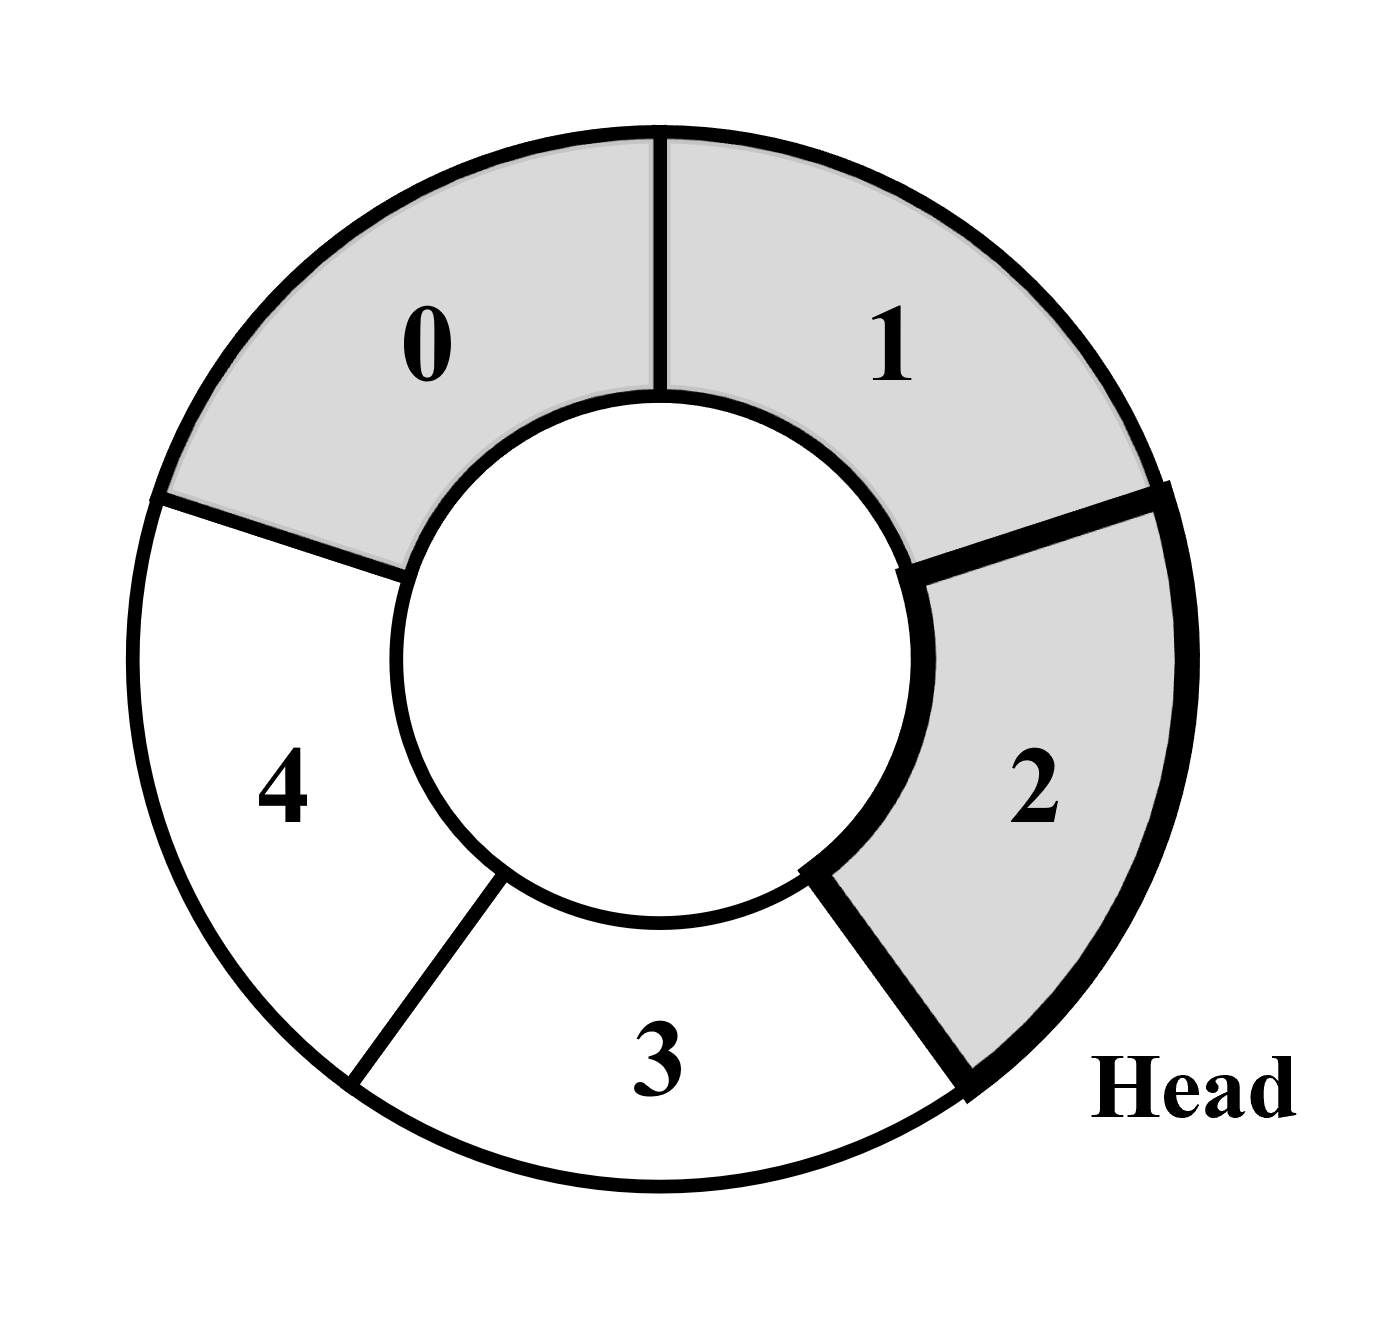
\includegraphics[height=0.9\textwidth]{07_stack0.png}
            \caption{Filling stack}
        \end{subfigure}
        \begin{subfigure}[t]{0.32\textwidth}
            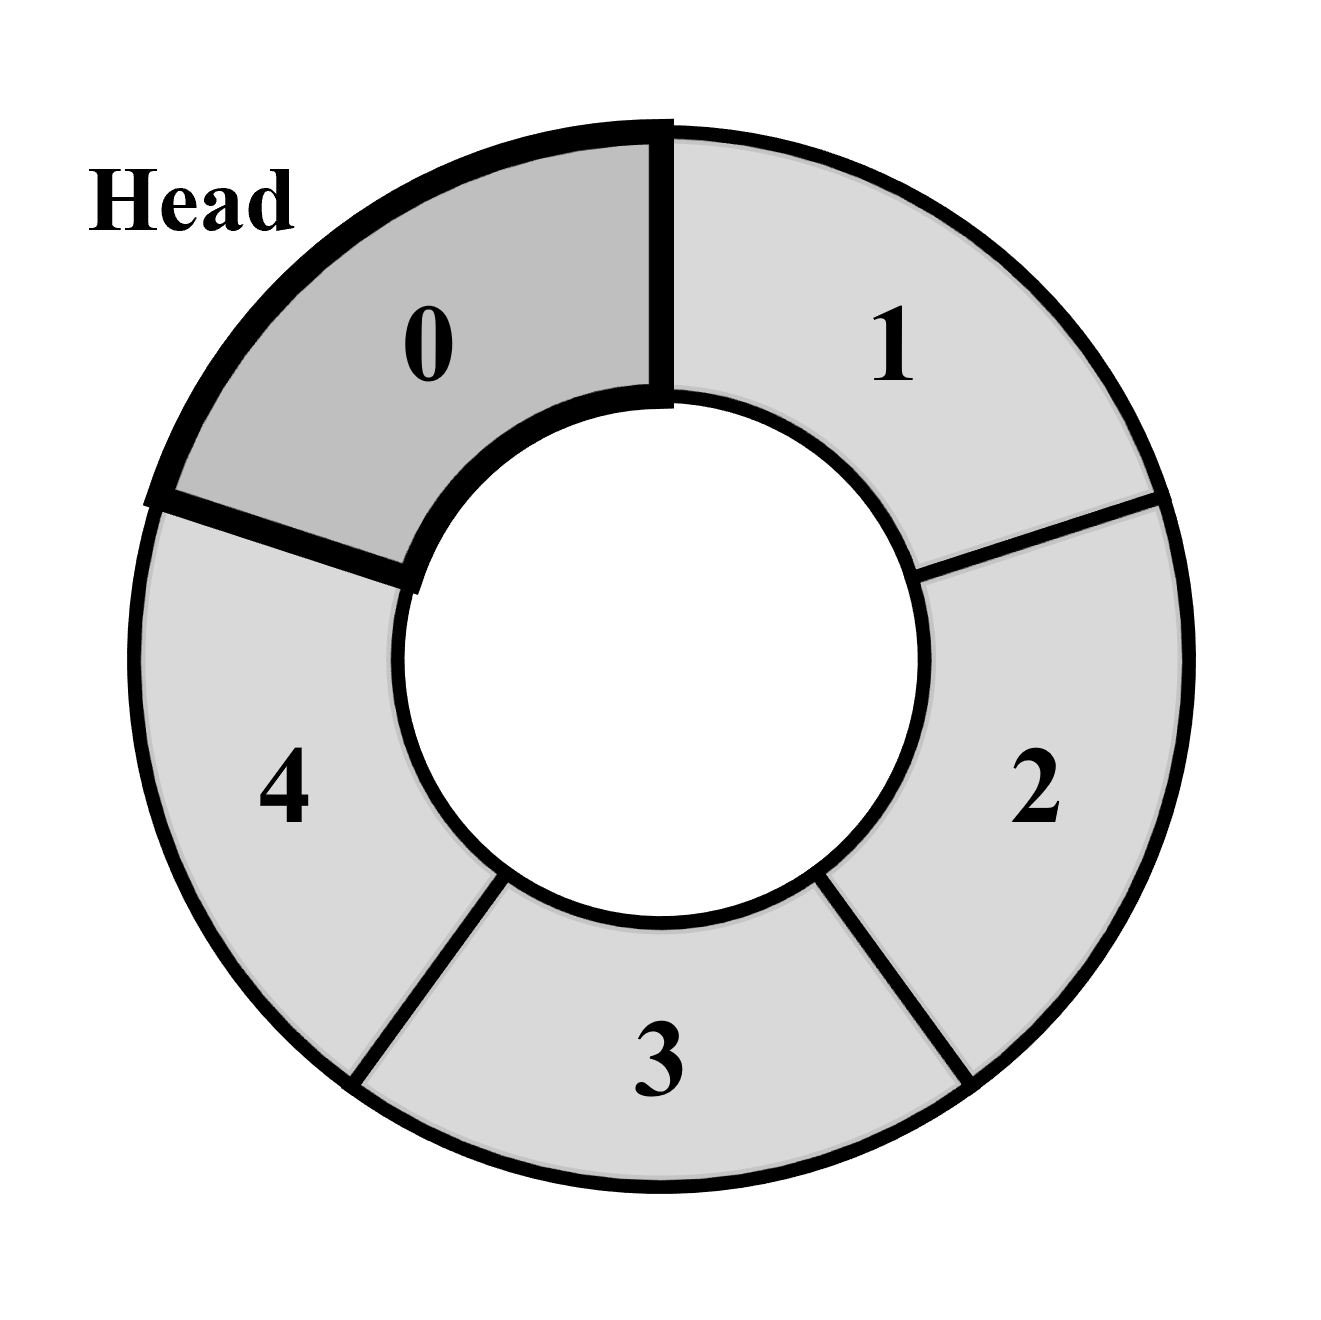
\includegraphics[height=0.9\textwidth]{07_stack1.png}
            \caption{Overwriting stack}
        \end{subfigure}
        \begin{subfigure}[t]{0.32\textwidth}
            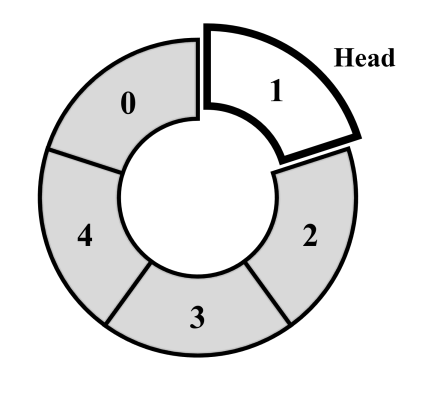
\includegraphics[height=0.9\textwidth]{07_stack2.png}
            \caption{Reading stack}
        \end{subfigure}
        \caption{TODO:}\label{fig:circleStack}
    \end{figure}

- Web workers, what are they? why are they needed?
- Communication channels
- Registry of topics/subs/pubs
- Message handling
width

\chapter{Package Management and Distribution}\label{cha:packages}

- Automating package building
- robostack?

\chapter{Concept Assessment}\label{cha:assessment}

- Survey
- Performance measures
- Limitations

\section{Levels}

    \subsection{Interaction}

        The scenario described is illustrated in Figure~\ref{fig:ui1}.

        \begin{figure}[htbp]
            \centering
            % \begin{tikzpicture}
            %     \draw[black, dashed, thin, fill=black!5] (0,0) rectangle (\linewidth,4);
            % \end{tikzpicture}
            \begin{lstlisting}[language=Bash]
Publisher initializing.
[INFO] [168766.57900] [wasm_cpp]: Context initializing.
[INFO] [168767.91500] [wasm_publisher]: Publishing: 'Hello there! 0'
[INFO] [168768.98400] [wasm_publisher]: Publishing: 'Hello there! 1'
[INFO] [168769.94400] [wasm_publisher]: Publishing: 'Hello there! 2'
[INFO] [168770.90300] [wasm_publisher]: Publishing: 'Hello there! 3'
[INFO] [168771.96800] [wasm_publisher]: Publishing: 'Hello there! 4'
[INFO] [168772.92000] [wasm_publisher]: Publishing: 'Hello there! 5'
[INFO] [168773.97600] [wasm_publisher]: Publishing: 'Hello there! 6'
[INFO] [168774.93600] [wasm_publisher]: Publishing: 'Hello there! 7'
\end{lstlisting}
            \caption{Output from non-interactive Level 1.}\label{fig:ui1}
        \end{figure}

        \begin{tcolorbox}[title=Example 1]
            \begin{minipage}[t]{0.87\linewidth}
                \vspace*{0pt}
                A demonstration of a \textit{non-interactive} user interface (Level 1) can
                be found at \href{https://ros2wasm.dev/pages/demo01/index.html}{\textsf{ros2wasm.dev/pages/demo01}}

                \textsc{Note:} The page must be reloaded to restart the node.
            \end{minipage}\hfill%
            \begin{minipage}[t]{0.1\linewidth}
                \vspace*{0pt}
                
\includegraphics[height=\linewidth,width=\linewidth]{qr_demo01.png}
            \end{minipage}
        \end{tcolorbox}


        Level 2 is exhibited in Figure~\ref{fig:ui2}

        \begin{figure}[htbp]
            \centering
            % 
\includegraphics[width=\linewidth]{03_level2.png}
            \begin{tikzpicture}
                \node (start) [
                    box,
                    xshift = -5cm,
                    minimum width = 2.5cm,
                ] {\footnotesize{\textbf{START}}};
                \node (stop) [
                    box,
                    minimum width = 2.5cm,
                    fill = igmrLightBlue,
                ] {\footnotesize{\textbf{STOP}}};
                \node (clear) [
                    box,
                    xshift = 5cm,
                    minimum width = 2.5cm,
                ] {\footnotesize{\textbf{CLEAR}}};
            \end{tikzpicture}
            \begin{lstlisting}[language=Bash]
[INFO] [16879468.55200] [wasm_publisher]: Publishing: 'Hello there! 13'
[INFO] [16879469.60800] [wasm_publisher]: Publishing: 'Hello there! 14'
[INFO] [16879470.56000] [wasm_publisher]: Publishing: 'Hello there! 15'
[INFO] [16879471.61600] [wasm_publisher]: Publishing: 'Hello there! 16'
[INFO] [16879472.56800] [wasm_publisher]: Publishing: 'Hello there! 17'
[INFO] [16879473.62400] [wasm_publisher]: Publishing: 'Hello there! 18'
Publisher terminated.\end{lstlisting}
            \caption{Interactive buttons to start and stop the publisher node.}\label{fig:ui2}
        \end{figure}

        \begin{tcolorbox}[title=Example 2]
            \begin{minipage}[t]{0.87\linewidth}
                \vspace*{0.5\baselineskip}
                A demonstration of a \textit{minimal} user interface (Level 2) can
                be found at \href{https://ros2wasm.dev/pages/demo02/index.html}{\textsf{ros2wasm.dev/pages/demo02}}
            \end{minipage}\hfill%
            \begin{minipage}[t]{0.1\linewidth}
                \vspace*{0pt}
                
\includegraphics[height=\linewidth,width=\linewidth]{qr_demo02.png}
            \end{minipage}
        \end{tcolorbox}

        Figure~\ref{fig:ui3} demonstrates a snapshot of Level 3.

        \begin{figure}[htbp]
            \centering
            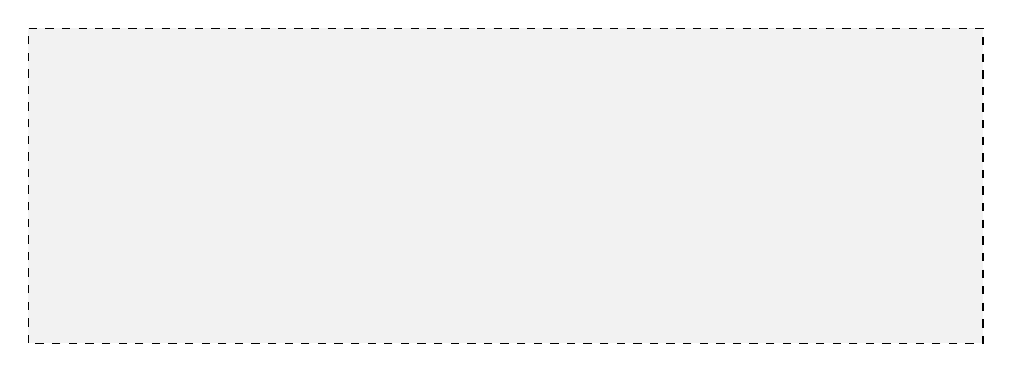
\begin{tikzpicture}
                \draw[black, dashed, thin, fill=black!5] (0,0) rectangle (\linewidth,4);
                \end{tikzpicture}
            \caption{TODO Level 3 image}\label{fig:ui3}
        \end{figure}

        \begin{tcolorbox}[title=Example 3]
            \begin{minipage}[t]{0.87\linewidth}
                \vspace*{0.5\baselineskip}
                A demonstration of a \textit{basic} user interface (Level 3) can
                be found at \href{https://ros2wasm.dev/pages/demo03/index.html}{\textsf{ros2wasm.dev/pages/demo03}}
            \end{minipage}\hfill%
            \begin{minipage}[t]{0.1\linewidth}
                \vspace*{0pt}
                
\includegraphics[height=\linewidth,width=\linewidth]{qr_demo03.png}
            \end{minipage}
        \end{tcolorbox}

        A depiction of Level 4 is shown in Figure~\ref{fig:ui4}

        \begin{figure}[htbp]
            \centering
            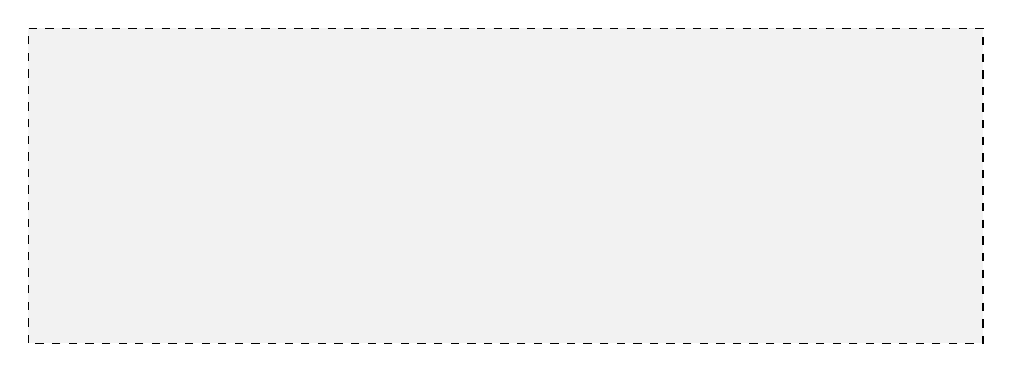
\begin{tikzpicture}
                \draw[black, dashed, thin, fill=black!5] (0,0) rectangle (\linewidth,4);
                \end{tikzpicture}
            \caption{TODO Level 4 image}\label{fig:ui4}
        \end{figure}

        \begin{tcolorbox}[title=Example 4]
            \begin{minipage}[t]{0.87\linewidth}
                \vspace*{0.5\baselineskip}
                A demonstration of an \textit{intermediate} user interface (Level 4) can
                be found at \href{https://ros2wasm.dev/pages/demo04/index.html}{\textsf{ros2wasm.dev/pages/demo04}}
            \end{minipage}\hfill%
            \begin{minipage}[t]{0.1\linewidth}
                \vspace*{0pt}
                
\includegraphics[height=\linewidth,width=\linewidth]{qr_demo04.png}
            \end{minipage}
        \end{tcolorbox}

        A typical workspace in JupyterLite is pictured in Figure~\ref{fig:ui5}.

        \begin{figure}[htbp]
            \centering
            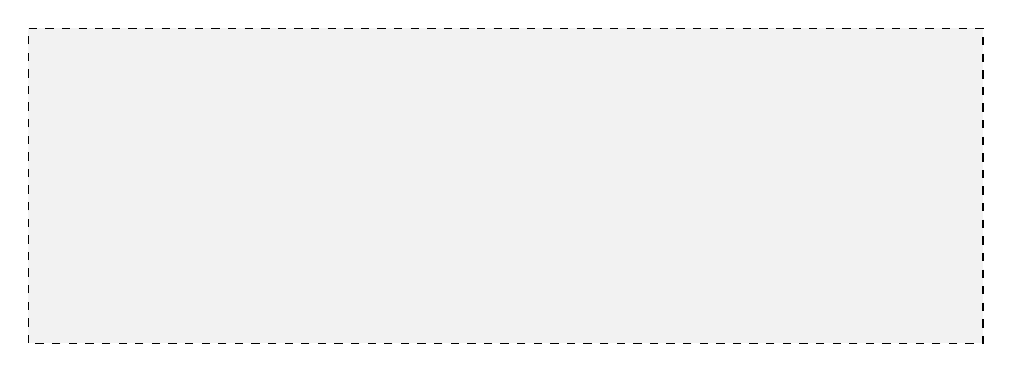
\begin{tikzpicture}
                \draw[black, dashed, thin, fill=black!5] (0,0) rectangle (\linewidth,4);
                \end{tikzpicture}
            \caption{TODO Level 5 image}\label{fig:ui5}
        \end{figure}

        % NO DEMO HERE
        % \begin{tcolorbox}[title=Example 5]
        %     \begin{minipage}[t]{0.87\linewidth}
        %         \vspace*{0.5\baselineskip}
        %         A demonstration of an \textit{advanced} user interface (Level 5) can
        %         be found at \href{https://ros2wasm.dev/pages/demo05/index.html}{\textsf{ros2wasm.dev/pages/demo05}}
        %     \end{minipage}\hfill%
        %     \begin{minipage}[t]{0.1\linewidth}
        %         \vspace*{0pt}
        %         
\includegraphics[height=\linewidth,width=\linewidth]{qr_demo05.png}
        %     \end{minipage}
        % \end{tcolorbox}


\chapter{Summary}\label{cha:summary}

\chapter{Outlook}\label{cha:outlook}

- Compiling on the browser
- Packaging Gazebo
- WASI

%%%%%%%%%%%%%%%%%%%%%%%%%%%%%%%%%%%%%%%%%%%%%%%%%%%%%%%%%%%%%%%%%%%%%%%%%%%%
%%%%%%%%%%%%%%%%%%%%%%%%%%%%%%%%%%%%%%%%%%%%%%%%%%%%%%%%%%%%%%%%%%%%%%%%%%%%
%%%%%%%%%%%%%%%%%%%%%%%%%%%%%%%%%%%%%%%%%%%%%%%%%%%%%%%%%%%%%%%%%%%%%%%%%%%%

\pagenumbering{Roman}
% --------------------------------------------------------------------------
%		Literaturverzeichnis / List of literature	
% -------------------------------------------------------------------------- 
\printbibliography[heading=bibintoc]

% --------------------------------------------------------------------------
%		Tabellenverzeichnis / List of tables
% -------------------------------------------------------------------------- 
\listoftables						% Tabellenverzeichnis / List of tables
\cleardoublepage

% --------------------------------------------------------------------------
%		Abbildungsverzeichnis / Register of illustrations
% -------------------------------------------------------------------------- 
\listoffigures						% Abbildungsverzeichnis / Register of illustrations
\cleardoublepage

% --------------------------------------------------------------------------
%		Anhang / Attachment
%
%		Der Anhnag enthält weitere Dokumente, welche nicht direkt zur Arbeit
%		gehören oder aus Platzgründen ausgelagert werden müssen. Die Kapitel
%		des Anhangs werden mit Großbuchstaben bezeichnet
%
%		The attachment contains further documents which are not related to work directly or
%		had to be outsourced due to a lack of space. The different chapters of the attachment 
%		are labeled with a captital letter.
% -------------------------------------------------------------------------- 
\appendix

% Inhalt des Anhangs (Beispiel) / List of contents of attachment (Example) 
\chapter{Illustrations}\label{cha:anhang_abbildungen}

\cleardoublepage
\chapter{Tables}\label{cha:anhang_tabellen}
\cleardoublepage

\chapter{Code}

\section{Build Script}\label{sec:apxblasm}

    \lstinputlisting[language=Bash]{05_appendix/blasm.sh}

    \pagebreak

\section{Build Workflow}\label{sec:apxworkflow}

    \lstinputlisting[language=Yaml]{05_appendix/workflow.yaml}

    \pagebreak

\section{rcutils Patch}\label{sec:apxpatch}

    \lstinputlisting[language=Bash]{05_appendix/rcutils.patch}

    \pagebreak

\section{JavaScript Functions}\label{sec:apxmodule}

    \lstinputlisting[language=JavaScript]{05_appendix/module.js}

    \pagebreak

% \section{RMW Adapter Function Headers}\label{sec:apxrmw}

%     \subsection{Initialization and Shutdown}
%         \lstinputlisting[language=C++]{05_appendix/rmwInit.cpp}

%     \subsection{Nodes}
%         \lstinputlisting[language=C++]{05_appendix/rmwNode.cpp}

%     \subsection{Implementation Information}
%         \lstinputlisting[language=C++]{05_appendix/rmwGetId.cpp}

%     \subsection{Publishers}
%         \lstinputlisting[language=C++]{05_appendix/rmwTopPub.cpp}

%     \subsection{Subscribers}
%         \lstinputlisting[language=C++]{05_appendix/rmwTopSub.cpp}
%         \lstinputlisting[language=C++]{05_appendix/rmwTopTake.cpp}

%     \subsection{Service Clients}
%         \lstinputlisting[language=C++]{05_appendix/rmwSrvClt.cpp}

%     \subsection{Service Servers}
%         \lstinputlisting[language=C++]{05_appendix/rmwSrvSrv.cpp}

%     \subsection{Guard Conditions}
%         \lstinputlisting[language=C++]{05_appendix/rmwGuard.cpp}
    
%     \pagebreak
%     \subsection{Wait Sets}
%         \lstinputlisting[language=C++]{05_appendix/rmwWait.cpp}

%     \subsection{Quality of Service}
%         \lstinputlisting[language=C++]{05_appendix/rmwQos.cpp}

%     \subsection{Serialization}
%         \lstinputlisting[language=C++]{05_appendix/rmwSerial.cpp}

%     \pagebreak
%     \subsection{Events}
%         \lstinputlisting[language=C++]{05_appendix/rmwEvents.cpp}

\backmatter
\end{document}